\chapter{樹與二元樹}
\label{ch:trees}

% 本章的圖共用的樣式與巨集（名稱都以 bt 開頭，避免和其他章衝突）
\tikzset{
    btn/.style={circle, draw=black!65, minimum size=6.5mm, inner sep=0pt, font=\small},
    bthl/.style={btn, fill=coreFill, draw=coreStroke},
    btop/.style={btn, fill=memFill, draw=memStroke},
    btthread/.style={-{Stealth[length=1.6mm]}, dashed, thick, draw=optStroke},
    bttree/.style={
        level distance=10mm,
        edge from parent/.style={draw=black!60, thick},
    },
    btmain/.style={bttree,
        level 1/.style={sibling distance=36mm},
        level 2/.style={sibling distance=18mm},
        level 3/.style={sibling distance=11mm},
        level 4/.style={sibling distance=9mm}},
}
% 本章大部分例子用的那棵樹（圖 7.1），節點名稱就是字母本身
\newcommand{\btmaintree}{%
\node[btn] (A) {A}
    child {node[btn] (B) {B}
        child {node[btn] (D) {D}}
        child {node[btn] (E) {E}
            child {node[btn] (G) {G}}
            child[missing]}}
    child {node[btn] (C) {C}
        child[missing]
        child {node[btn] (F) {F}
            child {node[btn] (H) {H}
                child[missing]
                child {node[btn] (J) {J}}}
            child {node[btn] (I) {I}}}};}

程式設計社的幹部名單要做成一張組織圖：社長底下有兩位副社長，每位副社長底下再各帶
幾個組長，組長底下還有組員。 這張圖不是一條直線，名單從社長開始往下分岔。 如果要
把它存進程式，之後還要「依職位由高到低列出所有人」或「從某個組長算起，他底下總共
有幾個人」，你會怎麼存？ 往下讀之前，先想一想。

前兩章的串列、堆疊和佇列都是\textbf{線性}的：每個元素最多只有一個「下一個」。 組
織圖、資料夾、比賽的對戰表、運算式的結構都是一層一層往下分岔的，這種結構叫
\textbf{樹}（tree）。 這一章先把名詞和幾個常考的性質整理清楚，再講二元樹的兩種存
法、四種走訪，以及考卷上最常見的幾種手算：由走訪序列把樹畫回來、在樹上加引線、數
有幾種不同形狀的二元樹、把運算式畫成樹。

這一章用到《C 程式設計基礎》第~14~章的結構指標、第~15~章的遞迴，以及第~19~章的
\texttt{malloc} 和二元樹入門（三種遍歷、由前序和中序重建）；用到時先在框裡複習。
本書第~6~章的堆疊、佇列和卡特蘭數，這一章會直接拿來用。

\section{名詞與基本性質}
\label{sec:bt-terms}

\subsection{樹的名詞}

一棵\textbf{樹}由有限個\textbf{節點}（node）組成。 不是空的樹有一個特別的節點叫
\textbf{根}（root），其餘的節點分成 $m \ge 0$ 組，每一組自己又是一棵樹，叫做根的
\textbf{子樹}（subtree）。 這個定義是遞迴的：樹是「一個根加上幾棵比較小的樹」。

根和每棵子樹的根之間連一條\textbf{邊}（edge）。 邊的上端叫\textbf{父節點}
（parent），下端叫\textbf{子節點}或\textbf{孩子}（child）；同一個父節點的孩子互為
\textbf{兄弟}（sibling）。 從根往下走到 $x$ 的路上經過的節點（含根，不含 $x$）是
$x$ 的\textbf{祖先}（ancestor），反過來 $x$ 是它們的\textbf{子孫}（descendant）。
除了根，每個節點恰好有一個父節點，所以 $n$ 個節點的樹恰好有 $n - 1$ 條邊。

一個節點的孩子個數叫它的\textbf{分支度}（degree）；整棵樹裡最大的分支度叫這棵樹的
分支度。 分支度為 $0$ 的節點是\textbf{葉節點}（leaf，也叫終端節點），其他的是
\textbf{內部節點}（internal node）。 好幾棵互不相交的樹放在一起叫\textbf{森林}
（forest）；把一棵樹的根拿掉，剩下的子樹就是一個森林。

孩子之間有先後順序（第一個孩子、第二個孩子……）的樹叫\textbf{有序樹}（ordered
tree）。 資料夾裡的項目、組織圖上由左到右的組別都有順序，本章的樹預設都是有序樹。

\subsection{深度、層與高度}

這三個詞各本書的定義不太一樣，本書固定用下面這一套：

\begin{itemize}
\item 節點 $x$ 的\textbf{深度}（depth）是從根走到 $x$ 經過的邊數，根的深度是 $0$。
\item 深度為 $d$ 的節點在第 $d + 1$ \textbf{層}（level），根在第 $1$ 層。
\item 樹的\textbf{高度}（height）是所有節點深度的最大值，也就是從根到最深的葉節點
經過的邊數。 只有一個節點的樹高度是 $0$，空樹的高度定為 $-1$。
\end{itemize}

所以高度為 $h$ 的樹共有 $h + 1$ 層。 有些書把「高度」定義成層數（只有根的樹高度是
$1$），有些書讓根在第 $0$ 層；同一個公式在不同定義下會差 $1$。

\begin{examnote}
題目問到高度、深度、層數，或「深度為 $k$ 的二元樹最多有幾個節點」這類公式時，先寫
一句「依題意，根在第 $1$ 層」或「這裡的高度是邊數」，再代公式。 題目沒有定義時，
寫出你用的定義，答案才不會因為差 $1$ 被當成錯的。 下面的「滿」「完整」也一樣，各
本書的用詞不同，先寫出定義。
\end{examnote}

\subsection{二元樹}

\begin{definition}[二元樹]
\label{def:bt-binary-tree}
一棵\textbf{二元樹}（binary tree）要嘛是空的，要嘛由一個根、一棵\textbf{左子樹}和
一棵\textbf{右子樹}組成，左右子樹各自也是二元樹（可以是空的）。
\end{definition}

二元樹和「分支度不超過 $2$ 的有序樹」不一樣：二元樹的孩子分左右，只有一個孩子時也
要說清楚是左孩子還是右孩子。 例如兩個節點的二元樹有兩種（根的左邊或右邊接一個節
點），兩個節點的有序樹只有一種。 二元樹也可以是空的，樹的定義通常不允許空樹。

圖~\ref{fig:bt-main} 是本章大部分例子用的二元樹，共 $10$ 個節點。 $A$ 是根；$B$、
$C$ 是 $A$ 的孩子；$C$ 只有右孩子 $F$；$D$、$G$、$J$、$I$ 是葉節點；$H$ 的深度是
$3$，在第 $4$ 層；這棵樹的高度是 $4$（$A \to C \to F \to H \to J$）。 $E$ 的祖先是
$B$、$A$，$F$ 的子孫是 $H$、$I$、$J$。

\begin{center}
\begin{tikzpicture}[btmain]
\btmaintree
\foreach \d/\y in {0/0, 1/-1, 2/-2, 3/-3, 4/-4} {
    \node[idxlbl, anchor=east] at (-4.6, \y) {深度 \d};
}
\end{tikzpicture}
\diagcaption{本章的例子樹 $T$。 分支度為 $2$ 的有 $A$、$B$、$F$，分支度為 $1$ 的有
$C$、$E$、$H$，其餘四個是葉節點。}
\label{fig:bt-main}
\end{center}

在正文裡畫樹很佔地方，所以本章也用一種文字寫法：$x(L, R)$ 表示根是 $x$、左子樹是
$L$、右子樹是 $R$，空的子樹寫 $-$，葉節點只寫名字。 圖~\ref{fig:bt-main} 的樹寫成
\[
A\bigl(B(D, E(G, -)),\; C(-, F(H(-, J), I))\bigr).
\]

\subsection{節點數與高度}

二元樹第 $1$ 層只有根，每往下一層，節點數最多變成兩倍，所以：

\begin{theorem}
\label{thm:bt-count}
\begin{enumerate}
\item 二元樹的第 $i$ 層最多有 $2^{i-1}$ 個節點（深度 $d$ 最多 $2^d$ 個）。
\item 高度為 $h$ 的二元樹最少有 $h + 1$ 個節點，最多有 $2^{h+1} - 1$ 個。
\item $n \ge 1$ 個節點的二元樹，高度 $h$ 滿足
$\lfloor \lg n \rfloor \le h \le n - 1$。
\end{enumerate}
\end{theorem}

\begin{proof}
(1) 對層數歸納：第 $1$ 層只有根，$2^0 = 1$。 第 $i$ 層的每個節點最多兩個孩子，所以
第 $i + 1$ 層最多 $2 \cdot 2^{i-1} = 2^i$ 個。

(2) 高度 $h$ 表示有一個深度 $h$ 的節點，它和它的 $h$ 個祖先就有 $h + 1$ 個節點。
最多的情形是每層都滿：$\sum_{d=0}^{h} 2^d = 2^{h+1} - 1$。

(3) 由 (2)，$n \le 2^{h+1} - 1 < 2^{h+1}$，取對數得 $\lg n < h + 1$。 $h$ 是整數，
所以 $h \ge \lfloor \lg n \rfloor$（若 $h < \lfloor \lg n \rfloor$，則
$h + 1 \le \lfloor \lg n \rfloor \le \lg n$，矛盾）。 上界由 (2) 的
$n \ge h + 1$ 得到。
\end{proof}

高度下界常寫成 $\lceil \lg(n + 1) \rceil - 1$，和 $\lfloor \lg n \rfloor$ 對所有
$n \ge 1$ 都相等。 第~9、10~章的搜尋樹每個操作都花 $\Theta(h)$，(3) 告訴我們 $h$ 最
好是 $\Theta(\lg n)$、最壞是 $\Theta(n)$，平衡樹要做的就是把 $h$ 壓在下界附近。

下一個性質是考卷上最常出現的一個等式。 令 $n_0$、$n_1$、$n_2$ 分別是分支度為
$0$、$1$、$2$ 的節點數。

\begin{theorem}
\label{thm:bt-n0n2}
不是空的二元樹都有 $n_0 = n_2 + 1$。
\end{theorem}

\begin{proof}
用兩種方式數邊。 每個節點都屬於三類之一，所以節點數 $n = n_0 + n_1 + n_2$，邊數是
$n - 1$。 另一方面，每條邊都是某個節點連到它的孩子，分支度 $1$ 的節點貢獻一條，分
支度 $2$ 的貢獻兩條，所以邊數也等於 $n_1 + 2 n_2$。 兩式相等：
$n_0 + n_1 + n_2 - 1 = n_1 + 2 n_2$，整理得 $n_0 = n_2 + 1$。
\end{proof}

圖~\ref{fig:bt-main} 的樹有 $n_2 = 3$、$n_0 = 4$，符合定理。 注意 $n_1$ 被消掉了：
分支度為 $1$ 的節點不管有幾個，都不影響葉節點的個數。 同樣的數邊法用在分支度最多
為 $k$ 的樹，令 $n_i$ 是分支度為 $i$ 的節點數，由
$\sum_i n_i - 1 = \sum_i i\, n_i$ 得到
\[
n_0 = 1 + \sum_{i=2}^{k} (i - 1)\, n_i = 1 + n_2 + 2 n_3 + \cdots + (k - 1) n_k .
\]

\subsection{滿二元樹、完整二元樹、嚴格二元樹}

有三種形狀特別常用，名稱在各本書差異很大，本書用的名稱和定義如下（英文名稱在不同書
裡也不一致，所以一併列出常見的叫法）：

\begin{center}
\begin{tabular}{p{0.2\linewidth}p{0.44\linewidth}p{0.26\linewidth}}
\toprule
本書用的名稱 & 定義 & 其他書的叫法 \\
\midrule
滿二元樹 & 每一層都是滿的；高度 $h$ 時恰有 $2^{h+1} - 1$ 個節點 & perfect binary tree；
有些書叫 full binary tree \\
完整二元樹 & 除了最後一層都是滿的，最後一層的節點都靠左邊 & complete binary tree；
也有人譯作完全二元樹 \\
嚴格二元樹 & 每個節點的分支度都是 $0$ 或 $2$ & CLRS 叫 full binary tree；也叫
proper binary tree \\
\bottomrule
\end{tabular}
\end{center}

\begin{center}
\begin{tikzpicture}[bttree, level 1/.style={sibling distance=18mm}, level 2/.style={sibling distance=9mm}]
\node[btn] {1}
    child {node[btn] {2} child {node[btn] {4}} child {node[btn] {5}}}
    child {node[btn] {3} child {node[btn] {6}} child {node[btn] {7}}};
\node at (0, -2.8) {\small 滿二元樹};
\begin{scope}[xshift=5cm]
\node[btn] {1}
    child {node[btn] {2} child {node[btn] {4}} child {node[btn] {5}}}
    child {node[btn] {3} child {node[btn] {6}} child[missing]};
\node at (0, -2.8) {\small 完整二元樹};
\end{scope}
\begin{scope}[xshift=10cm]
\node[btn] {}
    child {node[btn] {}}
    child {node[btn] {} child {node[btn] {}} child {node[btn] {}}};
\node at (0, -2.8) {\small 嚴格二元樹};
\end{scope}
\end{tikzpicture}
\diagcaption{三種特別的二元樹。 前兩棵的編號是由上到下、由左到右的順序，完整二元樹
的節點恰好是滿二元樹的編號 $1$ 到 $n$。}
\label{fig:bt-shapes}
\end{center}

完整二元樹的另一個說法是：把滿二元樹的節點由上到下、同一層由左到右編號 $1, 2,
\ldots$，$n$ 個節點的完整二元樹就是編號 $1$ 到 $n$ 的那些節點。 滿二元樹是完整二元
樹，反過來不一定。 嚴格二元樹由定理~\ref{thm:bt-n0n2} 有 $n_0 = n_2 + 1$、
$n_1 = 0$，所以節點數 $n = 2 n_2 + 1$ 一定是奇數。

\begin{theorem}
\label{thm:bt-complete-height}
$n$ 個節點的完整二元樹，高度是 $\lfloor \lg n \rfloor$；編號 $i$ 的節點深度是
$\lfloor \lg i \rfloor$。
\end{theorem}

\begin{proof}
深度 $d$ 那一層滿的時候，編號是 $2^d$ 到 $2^{d+1} - 1$（前 $d$ 層共 $2^d - 1$ 個節
點）。 所以編號 $i$ 的節點深度 $d$ 滿足 $2^d \le i < 2^{d+1}$，即
$d = \lfloor \lg i \rfloor$。 最深的節點是編號 $n$，高度是
$\lfloor \lg n \rfloor$。
\end{proof}

\section{表示法}
\label{sec:bt-repr}

\subsection{用陣列存}
\label{sec:bt-array}

把每個節點放在「它在滿二元樹裡的編號」那一格：根放 $A[1]$，編號 $i$ 的節點左孩子放
$A[2i]$、右孩子放 $A[2i + 1]$。 這樣父子關係都能用算的，不用存指標：

\begin{center}
\begin{tabular}{lll}
\toprule
 & 從 $1$ 開始（虛擬碼） & 從 $0$ 開始（C） \\
\midrule
父節點 & $\lfloor i / 2 \rfloor$（$i > 1$）& \texttt{(i - 1) / 2}（\texttt{i > 0}）\\
左孩子 & $2i$ & \texttt{2 * i + 1} \\
右孩子 & $2i + 1$ & \texttt{2 * i + 2} \\
\bottomrule
\end{tabular}
\end{center}

為什麼左孩子是 $2i$？ 由定理~\ref{thm:bt-complete-height} 的證明，深度 $d$ 那一層
的編號從 $2^d$ 開始。 編號 $i$ 是那一層的第 $i - 2^d$ 個（從 $0$ 數），它前面的
$i - 2^d$ 個節點在下一層各有兩個孩子，所以它的左孩子是下一層的第 $2(i - 2^d)$ 個，
編號 $2^{d+1} + 2(i - 2^d) = 2i$。 C 的版本是把每個編號減一：$2(i + 1) - 1 = 2i + 1$。

完整二元樹用這種存法剛好填滿 $A[1..n]$，一格都不浪費，第~8~章的堆積就是這樣存的。
不完整的樹就會有空格。 圖~\ref{fig:bt-main} 的樹存起來是：

\begin{center}
\setlength{\tabcolsep}{4pt}
\begin{tabular}{l*{15}{c}c}
\toprule
$i$ & 1 & 2 & 3 & 4 & 5 & 6 & 7 & 8 & 9 & 10 & 11 & 12 & 13 & 14 & 15 & $\cdots$ 29 \\
\midrule
$A[i]$ & A & B & C & D & E & & F & & & G & & & & H & I & $\cdots$ J \\
\bottomrule
\end{tabular}
\end{center}

$J$ 是 $H$（編號 $14$）的右孩子，編號 $29$，所以這棵 $10$ 個節點的樹要用 $29$ 格，
$16$ 到 $28$ 全空著。 最糟的是歪斜的樹（每個節點都只有右孩子）：$n$ 個節點的編號是
$1, 3, 7, \ldots, 2^n - 1$，要 $2^n - 1$ 格。 一般來說，高度 $h$ 的樹要準備
$2^{h+1} - 1$ 格。 另外，插入或刪除中間的節點時，整棵子樹的編號都要改，得搬很多
格。 所以陣列存法只適合完整（或接近完整）、形狀不常變的樹。

\subsection{用指標存}
\label{sec:bt-linked}

一般的二元樹用節點加指標存：每個節點有 $\mathit{key}$、$\mathit{left}$、
$\mathit{right}$，沒有的孩子是 \NIL；整棵樹用 $T.\mathit{root}$ 指向根，空樹時
$T.\mathit{root} = \NIL$。 需要從節點往上走時（例如第~9~章找後繼），再多存一個
$\mathit{parent}$。 這種存法每個節點的空間固定，插入、刪除只改幾個指標。

$n$ 個節點共有 $2n$ 個孩子指標，其中真的指向節點的恰好是邊數 $n - 1$ 個，所以有
\[
2n - (n - 1) = n + 1
\]
個指標是 \NIL，比一半還多。 第~\ref{sec:bt-thread}~節的引線二元樹就是要把這些空
指標拿來用。

\subsection{一般的樹：左孩子右兄弟}
\label{sec:bt-lcrs}

孩子個數不固定的樹（例如資料夾）怎麼存？ 直覺的做法是每個節點準備 $k$ 個孩子指標，
$k$ 是樹的分支度。 這很浪費：$n$ 個節點共 $nk$ 個指標，用到的只有 $n - 1$ 個，空指
標有 $n(k - 1) + 1$ 個；$k = 10$ 時九成以上的指標是空的。 而且 $k$ 要事先決定，有一
個資料夾特別大就全部跟著變大。

\textbf{左孩子右兄弟}（left-child, right-sibling）表示法只用兩個指標：
\begin{itemize}
\item $\mathit{child}$ 指向第一個（最左邊的）孩子；
\item $\mathit{sibling}$ 指向自己右邊的下一個兄弟。
\end{itemize}
一個節點的所有孩子從 $\mathit{child}$ 開始，沿著 $\mathit{sibling}$ 串成一條串列。
空指標只有 $n + 1$ 個，和二元樹一樣。

把 $\mathit{child}$ 看成左指標、$\mathit{sibling}$ 看成右指標，每一棵有序樹就變成一
棵二元樹，而且根沒有右孩子（根沒有兄弟）。 手算時用三個步驟：
\begin{enumerate}
\item 同一個父節點的孩子，由左到右用線連起來（兄弟相連）；
\item 每個節點只保留到第一個孩子的那條線，到其他孩子的線擦掉；
\item 原本往下的線當左指標、兄弟之間的線當右指標，順時針轉 $45^\circ$ 擺好。
\end{enumerate}

\begin{center}
\begin{tikzpicture}[bttree]
\begin{scope}[level 1/.style={sibling distance=20mm}, level 2/.style={sibling distance=9mm}]
\node[btn] (R) {R}
    child {node[btn] (P) {P} child {node[btn] (T) {T}} child {node[btn] (U) {U}}}
    child {node[btn] (Q) {Q}}
    child {node[btn] (S) {S} child {node[btn] (V) {V}} child {node[btn] (W) {W}} child {node[btn] (X) {X}}};
\draw[btthread, -] (P) -- (Q);
\draw[btthread, -] (Q) -- (S);
\draw[btthread, -] (T) -- (U);
\draw[btthread, -] (V) -- (W);
\draw[btthread, -] (W) -- (X);
\node at (0, -2.9) {\small 一般的樹（虛線是兄弟相連）};
\end{scope}
\begin{scope}[xshift=8.2cm, level 1/.style={sibling distance=20mm}, level 2/.style={sibling distance=14mm}, level 3/.style={sibling distance=10mm}, level 4/.style={sibling distance=9mm}, level distance=8.5mm]
\node[btn] {R}
    child {node[btn] {P}
        child {node[btn] {T} child[missing] child {node[btn] {U}}}
        child {node[btn] {Q}
            child[missing]
            child {node[btn] {S}
                child {node[btn] {V} child[missing] child {node[btn] {W} child[missing] child {node[btn] {X}}}}
                child[missing]}}}
    child[missing];
\node at (0, -5.9) {\small 對應的二元樹};
\end{scope}
\end{tikzpicture}
\diagcaption{左：一棵有序樹，$R$ 有三個孩子 $P$、$Q$、$S$。 右：左孩子右兄弟轉成的
二元樹，左指標是「第一個孩子」，右指標是「下一個兄弟」。 根 $R$ 沒有右孩子。}
\label{fig:bt-lcrs}
\end{center}

反過來，二元樹轉回一般的樹：每個節點 $x$ 的左孩子是 $x$ 的第一個孩子，從左孩子沿著
右指標一路走下去經過的節點，全都是 $x$ 的孩子。

\textbf{森林也可以轉成一棵二元樹}。 森林 $F = (T_1, T_2, \ldots, T_m)$ 對應的二元樹
$B(F)$ 遞迴定義如下：$m = 0$ 時是空樹；否則根是 $T_1$ 的根，左子樹是
$B(\text{$T_1$ 的根的子樹們})$，右子樹是 $B(T_2, \ldots, T_m)$。 手算的做法是先把每
棵樹各自轉好，再把 $T_2$ 的根接成 $T_1$ 的根的右孩子、$T_3$ 的根接成 $T_2$ 的根的右
孩子……，也就是把各棵樹的根當成兄弟。 轉回來的時候，從二元樹的根沿著右指標走，經過
的每個節點都是一棵樹的根。

\begin{center}
\begin{tikzpicture}[bttree]
\begin{scope}[level 1/.style={sibling distance=9mm}]
\node[btn] {A} child {node[btn] {B}} child {node[btn] {C}} child {node[btn] {D}};
\end{scope}
\begin{scope}[xshift=2.2cm]
\node[btn] {E} child {node[btn] {F}};
\end{scope}
\begin{scope}[xshift=4.0cm, level 1/.style={sibling distance=10mm}, level 2/.style={sibling distance=9mm}]
\node[btn] {G} child {node[btn] {H} child {node[btn] {I}} child[missing]} child {node[btn] {J}};
\end{scope}
\node at (2.0, -2.7) {\small 三棵樹的森林};
\begin{scope}[xshift=9.5cm, level 1/.style={sibling distance=30mm}, level 2/.style={sibling distance=14mm}, level 3/.style={sibling distance=10mm}, level distance=8.5mm]
\node[btn] {A}
    child {node[btn] {B} child[missing] child {node[btn] {C} child[missing] child {node[btn] {D}}}}
    child {node[btn] {E}
        child {node[btn] {F}}
        child {node[btn] {G}
            child {node[btn] {H} child {node[btn] {I}} child {node[btn] {J}}}
            child[missing]}};
\node at (0, -4.2) {\small 對應的二元樹};
\end{scope}
\end{tikzpicture}
\diagcaption{森林轉成二元樹。 三棵樹的根 $A$、$E$、$G$ 沿著右指標串在一起；$H$ 的
左孩子 $I$ 是它的第一個孩子，$H$ 的右孩子 $J$ 是它的下一個兄弟。}
\label{fig:bt-forest}
\end{center}

\textbf{走訪的對應}（第~\ref{sec:bt-walk}~節定義前序、中序、後序）。 森林的
\textbf{前序}是：先拜訪 $T_1$ 的根，再用前序走 $T_1$ 的根的子樹們，最後用前序走
$T_2, \ldots, T_m$；\textbf{後序}是：先用後序走 $T_1$ 的根的子樹們，再拜訪 $T_1$ 的
根，最後用後序走 $T_2, \ldots, T_m$。 對照 $B(F)$ 的定義，根是 $T_1$ 的根，左子樹是
$T_1$ 的子樹們，右子樹是其餘的樹，由歸納法立刻得到：
\begin{itemize}
\item 森林的前序 $=$ $B(F)$ 的前序；
\item 森林的後序 $=$ $B(F)$ 的\textbf{中序}。
\end{itemize}
以圖~\ref{fig:bt-forest} 為例，森林的前序是 $A\,B\,C\,D\,E\,F\,G\,H\,I\,J$，後序是
$B\,C\,D\,A\,F\,E\,I\,H\,J\,G$，正好是右邊二元樹的前序和中序。 有些書把森林的後序叫
做森林的「中序」，就是因為這個對應。 二元樹的後序則沒有自然的對應：它會把 $T_1$
的根排在 $T_2, \ldots, T_m$ 所有節點的後面，在原來的森林裡不是任何一種常用的順序。

\textbf{只存父節點}。 如果只需要從節點往上走（例如找路徑、判斷兩個節點是不是在同
一棵樹），可以每個節點只存父節點，根的父節點記成 $0$ 或 \NIL；陣列
$\mathit{parent}[1..n]$ 就能存一整個森林。 第~13~章的互斥集合就是這樣存的。 缺點是
找孩子要掃過所有節點。

\section{走訪}
\label{sec:bt-walk}

\textbf{走訪}（traversal）是把每個節點都拜訪恰好一次。 串列只有一種自然的順序，二
元樹就有好幾種。 最常用的三種都是遞迴的，差別只在「拜訪根」排在走左子樹、右子樹的
前面、中間還是後面：

\begin{itemize}
\item \textbf{前序}（preorder）：根、左子樹、右子樹。
\item \textbf{中序}（inorder）：左子樹、根、右子樹。
\item \textbf{後序}（postorder）：左子樹、右子樹、根。
\end{itemize}

左子樹一律在右子樹前面；把左右對調的三種（例如「根、右、左」）偶爾也會用到，但考
卷上說的前序、中序、後序就是上面這三種。

\begin{pseudo}[label=alg:bt-walks]{三種走訪}
\Procedure{Preorder}{$x$}
    \If{$x \ne \NIL$}
        \State 拜訪 $x$
        \State \Call{Preorder}{$x.\mathit{left}$}
        \State \Call{Preorder}{$x.\mathit{right}$}
    \EndIf
\EndProcedure
\Statex
\Procedure{Inorder}{$x$}
    \If{$x \ne \NIL$}
        \State \Call{Inorder}{$x.\mathit{left}$}
        \State 拜訪 $x$
        \State \Call{Inorder}{$x.\mathit{right}$}
    \EndIf
\EndProcedure
\Statex
\Procedure{Postorder}{$x$}
    \If{$x \ne \NIL$}
        \State \Call{Postorder}{$x.\mathit{left}$}
        \State \Call{Postorder}{$x.\mathit{right}$}
        \State 拜訪 $x$
    \EndIf
\EndProcedure
\end{pseudo}

圖~\ref{fig:bt-main} 的樹：
\begin{center}
\begin{tabular}{ll}
\toprule
前序 & $A\;B\;D\;E\;G\;C\;F\;H\;J\;I$ \\
中序 & $D\;B\;G\;E\;A\;C\;H\;J\;F\;I$ \\
後序 & $D\;G\;E\;B\;J\;H\;I\;F\;C\;A$ \\
\bottomrule
\end{tabular}
\end{center}

\textbf{手算的方法。} 想像從根的左上方出發，貼著樹的外緣逆時針繞一圈（每個節點都
繞過去，空的子樹也當成一小段路繞過）。 每個節點會被經過三次：從它的左邊經過、從它
的下方經過（走完左子樹、要往右子樹去的時候）、從它的右邊經過。 前序是第一次經過時
寫下它，中序是第二次，後序是第三次。 這個方法的好處是三種順序可以一次寫出來，而且
不用在腦子裡記遞迴到哪一層。

另外有兩個檢查答案的方法：前序的第一個一定是根，後序的最後一個一定是根；中序裡根
的左邊恰好是左子樹的節點。 第~\ref{sec:bt-rebuild}~節由走訪序列重建樹，用的就是這
兩件事。

\textbf{時間與空間。} 對有 $n$ 個節點的樹呼叫一次 \proc{Inorder}，每個節點會被呼叫
一次，每個 \NIL 指標也會被呼叫一次（立刻返回）。 由第~\ref{sec:bt-linked}~節，
\NIL 指標有 $n + 1$ 個，所以總共呼叫 $2n + 1$ 次，每次除了遞迴呼叫之外只做常數個步
驟，時間是 $\Theta(n)$。 另外兩種一樣。 遞迴最深時，呼叫堆疊上是從根到最深節點的
一條路徑，再加一個 \NIL，所以額外空間是 $\Theta(h)$：平衡的樹是 $\Theta(\lg n)$，歪
斜的樹是 $\Theta(n)$。

\subsection{C 程式：社團組織圖}

\begin{cbookrecap}[第~14~章 14.5 節、第~15~章 15.10 節、第~19~章 19.14--19.17 節]
節點的結構裡有兩個指向同型結構的指標：\texttt{struct Node *left, *right;}，所以要先
寫 \texttt{typedef struct Node \{ ... \} Node;} 的完整標籤，結構裡面才能用
\texttt{struct Node}。 第~15~章說過，資料的定義是遞迴的（樹要嘛是 \texttt{NULL}，
要嘛是一個節點接上兩棵樹），函式就照著寫：先處理 \texttt{NULL}，再處理
\texttt{t->left} 和 \texttt{t->right}。 第~19~章 19.16 節的三種遍歷只差
\texttt{printf} 放在兩個遞迴呼叫的前、中、後；19.17 節用前序和中序重建過二元樹。

釋放整棵樹要用後序：先釋放兩棵子樹，最後才 \texttt{free(t)}。 先 \texttt{free(t)}
的話，之後再讀 \texttt{t->left} 就是讀已經釋放的記憶體。
\end{cbookrecap}

程式設計社的幹部用一個大寫字母代表，組織圖存成二元樹。 樹用\textbf{延伸前序}輸入：
照前序寫出每個節點，空的子樹也寫成一個 \texttt{.}，這樣一個序列就能唯一決定一棵樹
（第~\ref{sec:bt-rebuild}~節說明）。 圖~\ref{fig:bt-main} 的樹寫成
\texttt{ABD..EG...C.FH.J..I..}，$10$ 個字母加 $11$ 個點，點的個數正好是 \NIL 指標的
個數 $n + 1$。 程式印出三種走訪、高度，以及分支度 $0$、$1$、$2$ 的節點數，用來驗證定
理~\ref{thm:bt-n0n2}。

\begin{example}[label=ex:bt-club]{c}{(club\_tree.c) 社團組織圖的三種走訪}
#include <stdio.h>
#include <stdlib.h>

typedef struct Node {
    char key;                   // 幹部代號，一個大寫字母
    struct Node *left, *right;
} Node;

// 從延伸前序建樹：字母是節點，'.' 是空的子樹，*pos 是讀到的位置
Node *build(const char *s, int *pos)
{
    char c = s[*pos];
    if (c == '\0') {            // 字串不夠長：當成空的
        return NULL;
    }
    (*pos)++;
    if (c == '.') {
        return NULL;
    }
    Node *p = malloc(sizeof *p);
    if (p == NULL) {
        exit(1);
    }
    p->key = c;
    p->left = build(s, pos);    // 先讀完整個左子樹
    p->right = build(s, pos);
    return p;
}

// when 是 0、1、2：在走左子樹之前、之間、之後印出根（前序、中序、後序）
void walk(const Node *t, int when)
{
    if (t == NULL) {
        return;
    }
    if (when == 0) {
        printf(" %c", t->key);
    }
    walk(t->left, when);
    if (when == 1) {
        printf(" %c", t->key);
    }
    walk(t->right, when);
    if (when == 2) {
        printf(" %c", t->key);
    }
}

int height(const Node *t)       // 邊數；空樹是 -1
{
    if (t == NULL) {
        return -1;
    }
    int hl = height(t->left), hr = height(t->right);
    return 1 + (hl > hr ? hl : hr);
}

void count_degree(const Node *t, int cnt[3])    // cnt[d]：分支度 d 的個數
{
    if (t != NULL) {
        cnt[(t->left != NULL) + (t->right != NULL)]++;
        count_degree(t->left, cnt);
        count_degree(t->right, cnt);
    }
}

void free_tree(Node *t)         // 後序：孩子都釋放了才釋放自己
{
    if (t != NULL) {
        free_tree(t->left);
        free_tree(t->right);
        free(t);
    }
}

int main(void)
{
    char s[128];
    while (scanf("%127s", s) == 1) {
        int pos = 0, cnt[3] = {0, 0, 0};
        Node *root = build(s, &pos);
        const char *name[3] = {"pre", "in", "post"};
        printf("%s\n", s);
        for (int w = 0; w < 3; w++) {
            printf("%s:", name[w]);
            walk(root, w);
            printf("\n");
        }
        count_degree(root, cnt);
        printf("height %d, n0 %d, n1 %d, n2 %d\n", height(root), cnt[0], cnt[1], cnt[2]);
        free_tree(root);
    }
    return 0;
}
\end{example}
\iosample{ABD..EG...C.FH.J..I.. \\ A.B.C..}{ABD..EG...C.FH.J..I.. \\ pre: A B D E G C F H J I \\ in: D B G E A C H J F I \\ post: D G E B J H I F C A \\ height 4, n0 4, n1 3, n2 3 \\ A.B.C.. \\ pre: A B C \\ in: A B C \\ post: C B A \\ height 2, n0 1, n1 2, n2 0}

三種走訪寫成同一個函式 \texttt{walk}，參數 \texttt{when} 決定 \texttt{printf}
放在兩個遞迴呼叫的前、中、後。 \texttt{height} 要先知道兩棵子樹的高度才能算出自己
的，是後序；\texttt{free\_tree} 也是後序。 高度用邊數，所以空樹回傳 $-1$，葉節點得
到 $1 + \max(-1, -1) = 0$；題目把高度定義成層數時，空樹改回傳 $0$ 就好。 第二棵樹
$A(-, B(-, C))$ 是只往右長的鏈，前序和中序相同，高度是 $2$。 層序和迴圈版的走訪，下
面兩小節先講虛擬碼，C 的寫法留給實作練習的前幾題。

\subsection{層序走訪}
\label{sec:bt-level}

\textbf{層序}（level order）是一層一層、同一層由左到右拜訪。 層序沒有遞迴的寫法，
要用佇列（第~6~章）：先放進根；每次從佇列拿出一個節點，拜訪它，再把它的左、右孩子
依序放進佇列。

\begin{pseudo}[label=alg:bt-level]{層序走訪}
\Procedure{Level-Order}{$T$}
    \If{$T.\mathit{root} = \NIL$}
        \State \Return
    \EndIf
    \State 建立空佇列 $Q$
    \State \Call{Enqueue}{$Q, T.\mathit{root}$}
    \While{$Q$ 不是空的}
        \State $x \gets$ \Call{Dequeue}{$Q$}
        \State 拜訪 $x$
        \If{$x.\mathit{left} \ne \NIL$}
            \State \Call{Enqueue}{$Q, x.\mathit{left}$}
        \EndIf
        \If{$x.\mathit{right} \ne \NIL$}
            \State \Call{Enqueue}{$Q, x.\mathit{right}$}
        \EndIf
    \EndWhile
\EndProcedure
\end{pseudo}

用圖~\ref{fig:bt-main} 的樹走一次，每一列是一次 \proc{Dequeue}：

\begin{center}
\begin{tabular}{ccl}
\toprule
拿出並拜訪 & 放進佇列 & 之後的佇列（前 $\to$ 後）\\
\midrule
$A$ & $B$, $C$ & $B\;C$ \\
$B$ & $D$, $E$ & $C\;D\;E$ \\
$C$ & $F$ & $D\;E\;F$ \\
$D$ & & $E\;F$ \\
$E$ & $G$ & $F\;G$ \\
$F$ & $H$, $I$ & $G\;H\;I$ \\
$G$ & & $H\;I$ \\
$H$ & $J$ & $I\;J$ \\
$I$ & & $J$ \\
$J$ & & （空）\\
\bottomrule
\end{tabular}
\end{center}

為什麼這樣會一層一層出來？ 佇列裡的節點，深度由前到後不會減少，而且最多只差一層：
拿出深度 $d$ 的節點時放進去的是深度 $d + 1$ 的節點，排在所有已經在佇列裡的節點後
面。 同一層裡，左邊節點的孩子先進佇列，所以也先出來。 每個節點進出佇列各一次，時
間 $\Theta(n)$；佇列最長時大約是最寬的那一層，完整二元樹的最後一層可以有大約 $n/2$
個節點。 第~21~章的廣度優先搜尋就是把層序推廣到圖上。

\subsection{不用遞迴的走訪}
\label{sec:bt-iter}

第~6~章 6.4 節說過，任何遞迴都能改寫成迴圈加上自己管理的堆疊。 樹很深的時候（例如
十萬個節點排成一條鏈），遞迴版會用完系統的呼叫堆疊，這時就需要迴圈版。

\textbf{中序。} 遞迴版進到一個節點時，要先把左子樹整個做完，才輪到它自己，所以「它
自己」要先存起來。 迴圈版從根開始一路往左走，路上的節點都 push 進堆疊；走到底之
後，pop 出來的那個就是下一個要拜訪的（它的左子樹已經做完了），拜訪它，再轉到它的
右子樹，重複同樣的事。

\begin{pseudo}[label=alg:bt-inorder-iter]{中序走訪的迴圈版}
\Procedure{Inorder-Iter}{$T$}
    \State 建立空堆疊 $S$
    \State $x \gets T.\mathit{root}$
    \While{$x \ne \NIL$ \OR $S$ 不是空的}
        \While{$x \ne \NIL$} \Comment{一路往左，路上的節點先存著}
            \State \Call{Push}{$S, x$}
            \State $x \gets x.\mathit{left}$
        \EndWhile
        \State $x \gets$ \Call{Pop}{$S$} \Comment{它的左子樹已經做完}
        \State 拜訪 $x$
        \State $x \gets x.\mathit{right}$
    \EndWhile
\EndProcedure
\end{pseudo}

用圖~\ref{fig:bt-main} 的樹追蹤，每一列是一次拜訪，「推入」是拜訪前第 5--7 行
push 的節點：

\begin{center}
\begin{tabular}{ccl}
\toprule
拜訪 & 拜訪前推入 & 拜訪後的堆疊（底 $\to$ 頂）\\
\midrule
$D$ & $A, B, D$ & $A\;B$ \\
$B$ & & $A$ \\
$G$ & $E, G$ & $A\;E$ \\
$E$ & & $A$ \\
$A$ & & （空）\\
$C$ & $C$ & （空）\\
$H$ & $F, H$ & $F$ \\
$J$ & $J$ & $F$ \\
$F$ & & （空）\\
$I$ & $I$ & （空）\\
\bottomrule
\end{tabular}
\end{center}

拜訪的順序就是中序。 注意 push 的順序是 $A, B, D, E, G, C, F, H, J, I$，正好是前
序：這不是巧合，第~\ref{sec:bt-count}~節會用到這件事。 堆疊裡的節點永遠在同一條從
根往下的路徑上，所以最多 $h + 1$ 個（觀念題第~\ref{q:bt-stack-height}~題）。

\textbf{前序。} 前序比較簡單：pop 出一個節點就拜訪它，再把右孩子、左孩子依序 push。
左孩子後放，所以先出來，整個左子樹會在右孩子 pop 出來之前做完。 這就是第~6~章「把
子工作倒過來 push」的規則。

\textbf{後序。} 後序最麻煩：一個節點要等左右子樹都做完才能拜訪，而它從堆疊頂端被
看到的時候，可能是剛做完左子樹（還要去右子樹），也可能是剛做完右子樹（該拜訪它了）。
分辨的方法是記住上一個拜訪的節點 $\mathit{last}$：頂端節點的右孩子存在而且不是
$\mathit{last}$，表示右子樹還沒做；否則就拜訪它、pop 掉。

\begin{pseudo}[label=alg:bt-postorder-iter]{後序走訪的迴圈版}
\Procedure{Postorder-Iter}{$T$}
    \State 建立空堆疊 $S$
    \State $x \gets T.\mathit{root}$，$\mathit{last} \gets \NIL$
    \While{$x \ne \NIL$ \OR $S$ 不是空的}
        \While{$x \ne \NIL$}
            \State \Call{Push}{$S, x$}
            \State $x \gets x.\mathit{left}$
        \EndWhile
        \State $p \gets$ \Call{Top}{$S$} \Comment{先看，不拿}
        \If{$p.\mathit{right} \ne \NIL$ \AND $p.\mathit{right} \ne \mathit{last}$}
            \State $x \gets p.\mathit{right}$ \Comment{右子樹還沒做}
        \Else
            \State 拜訪 $p$
            \State $\mathit{last} \gets p$
            \State \Call{Pop}{$S$}
        \EndIf
    \EndWhile
\EndProcedure
\end{pseudo}

第 9 行為什麼可以只比較右孩子？ 頂端節點 $p$ 被第二次看到時，剛做完的一定是它的
某棵子樹，而子樹做完時最後拜訪的就是子樹的根（後序最後才拜訪根）。 所以剛做完右子
樹時 $\mathit{last} = p.\mathit{right}$；剛做完左子樹時，$\mathit{last}$ 是
$p.\mathit{left}$（或在 $p$ 沒有左孩子時是更早的節點），不會等於
$p.\mathit{right}$。

\section{由走訪序列重建}
\label{sec:bt-rebuild}

只給一種走訪序列，畫不出唯一的樹：前序 $A\,B$ 可以是 $A(B, -)$，也可以是
$A(-, B)$。 考卷上常給兩種序列，要你把樹畫回來。 這一節假設節點的名稱互不相同。

\subsection{前序加中序}

前序的第一個是根。 在中序裡找到根，它左邊的是左子樹的節點、右邊的是右子樹的節點，
個數也就知道了。 前序在根之後，先是整個左子樹、再是整個右子樹，所以照左子樹的個數
就能把前序切成兩段。 兩邊各自又是「前序加中序」，遞迴下去。

\begin{theorem}
\label{thm:bt-pre-in}
節點名稱互不相同時，前序和中序可以唯一決定一棵二元樹。 後序和中序也可以。
\end{theorem}

\begin{proof}
對節點數 $n$ 做強歸納。 $n = 0$ 只有空樹。 $n \ge 1$ 時，設兩棵樹 $T$、$T'$ 的前序
都是 $p_1 \cdots p_n$、中序都是 $q_1 \cdots q_n$。 兩棵樹的根都是 $p_1$。 設 $p_1 =
q_k$；名稱互不相同，$k$ 是唯一的。 中序是「左子樹、根、右子樹」，所以兩棵樹的左子
樹都由 $q_1 \cdots q_{k-1}$ 組成，中序就是這一串；右子樹的中序都是
$q_{k+1} \cdots q_n$。 左子樹有 $k - 1$ 個節點，前序是「根、左子樹、右子樹」，所以
兩棵樹的左子樹前序都是 $p_2 \cdots p_k$，右子樹前序都是 $p_{k+1} \cdots p_n$。 兩
棵左子樹的前序、中序都相同，節點數小於 $n$，由歸納假設是同一棵；右子樹也一樣。 所
以 $T = T'$。 後序加中序的證明相同，只是根改成後序的最後一個。
\end{proof}

這個證明本身就是演算法。 用一個表 $\mathit{pos}[c]$ 記住名稱 $c$ 在中序裡的位置，找
根就是 $\Theta(1)$：

\begin{pseudo}[label=alg:bt-pre-in]{由前序和中序建樹}
\Function{Build-Pre-In}{$i, j, m$} \Comment{$\mathit{pre}[i..i{+}m{-}1]$ 和 $\mathit{in}[j..j{+}m{-}1]$ 是同一棵子樹}
    \If{$m = 0$}
        \State \Return \NIL
    \EndIf
    \State $k \gets \mathit{pos}[\mathit{pre}[i]]$ \Comment{根在中序的位置}
    \State $\ell \gets k - j$ \Comment{左子樹的節點數}
    \State 配置新節點 $x$，$x.\mathit{key} \gets \mathit{pre}[i]$
    \State $x.\mathit{left} \gets$ \Call{Build-Pre-In}{$i + 1, j, \ell$}
    \State $x.\mathit{right} \gets$ \Call{Build-Pre-In}{$i + 1 + \ell, k + 1, m - 1 - \ell$}
    \State \Return $x$
\EndFunction
\end{pseudo}

每個節點建一次，每次 $\Theta(1)$，總時間 $\Theta(n)$。 不用 $\mathit{pos}$ 表、每次
在中序裡從頭找根的話，最壞（歪斜的樹）是 $\Theta(n^2)$。

\textbf{手算追蹤。} 前序 $A\,B\,D\,E\,G\,C\,F\,H\,J\,I$、中序
$D\,B\,G\,E\,A\,C\,H\,J\,F\,I$。 每一列處理一棵子樹：

\begin{center}
\begin{tabular}{llcll}
\toprule
子樹的前序 & 子樹的中序 & 根 & 左子樹（中序）& 右子樹（中序）\\
\midrule
$ABDEGCFHJI$ & $DBGE\,|\,A\,|\,CHJFI$ & $A$ & $DBGE$ & $CHJFI$ \\
$BDEG$ & $D\,|\,B\,|\,GE$ & $B$ & $D$ & $GE$ \\
$EG$ & $G\,|\,E$ & $E$ & $G$ & 空 \\
$CFHJI$ & $C\,|\,HJFI$ & $C$ & 空 & $HJFI$ \\
$FHJI$ & $HJ\,|\,F\,|\,I$ & $F$ & $HJ$ & $I$ \\
$HJ$ & $H\,|\,J$ & $H$ & 空 & $J$ \\
\bottomrule
\end{tabular}
\end{center}

只剩一個節點的子樹（$D$、$G$、$I$、$J$）不必再列。 由表就能畫出圖~\ref{fig:bt-main}
的樹。 切前序時要數個數：$A$ 的左子樹有 $4$ 個節點，所以前序 $A$ 後面的 $BDEG$ 是
左子樹，剩下的 $CFHJI$ 是右子樹。

\begin{examnote}
重建的題目，每一步寫出「根是誰、左子樹有哪些節點、右子樹有哪些節點」，像上面的表一
樣一棵子樹一列，最後再畫樹。 畫完之後用另一種走訪（例如後序）走一次自己畫的樹，和
題目給的序列核對；題目問「這樣的樹存不存在」時，矛盾出現在哪一步就寫哪一步。
\end{examnote}

\textbf{後序加中序}的做法對稱：根是後序的最後一個，左子樹有 $\ell$ 個節點時，後序
的前 $\ell$ 個是左子樹、接下來到倒數第二個是右子樹。 \textbf{層序加中序}也能唯一決定
樹：層序裡第一個出現的是根；切開中序之後，左子樹的層序就是整個層序裡屬於左子樹的那
些節點，順序不變（觀念題第~\ref{q:bt-level-in}~題）。

\subsection{前序加後序不夠}

前序和後序都不告訴你「哪些節點在左邊」。 最小的反例是兩個節點：
$A(B, -)$ 和 $A(-, B)$ 的前序都是 $A\,B$、後序都是 $B\,A$。 一般來說，問題出在只有
一個孩子的節點：前序、後序看得出它有一個孩子，看不出是左還是右。

用前序和後序還是可以找出每個節點有哪些孩子。 設某棵子樹的前序是 $x\,y \cdots$，則
$y$ 是 $x$ 的第一棵子樹的根；在後序裡，$y$ 的子樹以 $y$ 結尾，由 $y$ 的位置可以算出
這棵子樹有幾個節點。 如果它就是 $x$ 底下全部的節點，$x$ 只有一個孩子，左右無法決定；
否則 $x$ 有兩個孩子，$y$ 在左邊，另一棵子樹的根是前序裡接在 $y$ 的子樹後面的那一個。
所以：

\begin{theorem}
\label{thm:bt-pre-post}
節點名稱互不相同。 給定前序和後序，若至少有一棵二元樹符合，則符合的樹恰好有 $2^m$
棵，$m$ 是分支度為 $1$ 的節點個數（對每一棵符合的樹，$m$ 都一樣）。 特別地，嚴格二
元樹可以由前序和後序唯一決定。
\end{theorem}

證明留作觀念題第~\ref{q:bt-pre-post}~題。 例如前序 $A\,B\,C$、後序 $C\,B\,A$：$A$、
$B$ 都只有一個孩子，共 $2^2 = 4$ 棵，分別是 $B$ 接在 $A$ 的左或右、$C$ 接在 $B$ 的
左或右。

\textbf{延伸前序}也能唯一決定樹，因為它把每個節點的分支度和左右都寫進去了：讀到字
母就是一個節點，接著讀它的左子樹、再讀右子樹；讀到 \texttt{.} 就是空的子樹。 範
例~\ref{ex:bt-club} 的 \texttt{build} 就是照這個定義寫的。

\subsection{C 程式}

下面的程式讀入多組前序和中序，建好樹之後用後序印出來。 兩個序
列可能互相矛盾，例如前序 $A\,B\,C\,D$、中序 $B\,D\,A\,C$ 根本沒有對應的樹，程式要
能發現。 發現的方法很簡單：每次找到的根，在中序裡的位置必須落在目前這一段裡面。

\begin{example}[label=ex:bt-rebuild]{c}{(rebuild.c) 由兩種走訪序列重建}
#include <stdio.h>
#include <stdlib.h>
#include <string.h>

typedef struct Node {
    char key;
    struct Node *left, *right;
} Node;

static int pos[256];            // pos[c]：c 在中序裡的位置，不在就是 -1
static int ok;                  // 序列互相矛盾時設成 0

Node *new_node(char c)
{
    Node *p = malloc(sizeof *p);
    if (p == NULL) {
        exit(1);
    }
    p->key = c;
    p->left = p->right = NULL;
    return p;
}

// 前序 pre[pl..pl+n-1]、中序 in[il..il+n-1] 描述同一棵子樹
Node *from_pre_in(const char *pre, int pl, int il, int n)
{
    if (n == 0 || !ok) {
        return NULL;
    }
    int k = pos[(unsigned char)pre[pl]];    // 根在中序的位置
    if (k < il || k >= il + n) {            // 根不在這一段：矛盾
        ok = 0;
        return NULL;
    }
    int nl = k - il;                        // 左子樹的節點數
    Node *p = new_node(pre[pl]);
    p->left = from_pre_in(pre, pl + 1, il, nl);
    p->right = from_pre_in(pre, pl + 1 + nl, k + 1, n - 1 - nl);
    return p;
}

void postorder(const Node *t)
{
    if (t != NULL) {
        postorder(t->left);
        postorder(t->right);
        putchar(t->key);
    }
}

void free_tree(Node *t)
{
    if (t != NULL) {
        free_tree(t->left);
        free_tree(t->right);
        free(t);
    }
}

int main(void)
{
    char pre[64], in[64];
    while (scanf("%63s %63s", pre, in) == 2) {   // 每行：前序 中序
        int n = strlen(in);
        ok = (int)strlen(pre) == n;
        memset(pos, -1, sizeof pos);
        for (int i = 0; i < n; i++) {
            unsigned char c = in[i];
            if (pos[c] != -1) {
                ok = 0;                     // 中序裡有重複的字母
            }
            pos[c] = i;
        }
        Node *root = from_pre_in(pre, 0, 0, n);
        printf("pre %s, in %s -> ", pre, in);
        if (ok) {
            printf("post ");
            postorder(root);
            printf("\n");
        } else {
            printf("no such tree\n");
        }
        free_tree(root);
    }
    return 0;
}
\end{example}
\iosample{ABDEGCFHJI DBGEACHJFI \\ ABCD BADC \\ ABCD BDAC \\ ABC ABD}{pre ABDEGCFHJI, in DBGEACHJFI -> post DGEBJHIFCA \\ pre ABCD, in BADC -> post BDCA \\ pre ABCD, in BDAC -> no such tree \\ pre ABC, in ABD -> no such tree}

為什麼只要檢查「根落在這一段」就夠了？ 對子樹大小歸納：一段長度為 $1$ 時，根落在
這一段表示前序和中序的這個字母相同；長度更長時，左右兩段各自通過檢查，由歸納假設
建出來的左右子樹的中序分別是那兩段，接上根之後整棵樹的中序就是整段。 所以程式沒有
回報矛盾時，建出來的樹的前序和中序一定和輸入相同。 第三組在處理 $B$ 的右子樹時，前
序剩下 $C$、中序剩下 $D$，$C$ 不在這一段，所以回報 \texttt{no such tree}。 第四組
的前序裡有 $C$，中序裡卻沒有，\texttt{pos} 查到 $-1$，一樣不在範圍內。 後序加中序
的版本只要把根改成後序的最後一個，切法照上面說的改。

\section{引線二元樹}
\label{sec:bt-thread}

第~\ref{sec:bt-linked}~節算過，$n$ 個節點的二元樹有 $n + 1$ 個 \NIL 指標。 另一方
面，中序走訪的迴圈版要一個堆疊，遞迴版要呼叫堆疊，都要 $\Theta(h)$ 的額外空間。
\textbf{引線二元樹}（threaded binary tree）把這些空的指標拿來指向中序的前後節點，
走訪時就不需要堆疊了。

\subsection{中序引線}

\textbf{中序引線}的規則：
\begin{itemize}
\item 節點的左指標原本是 \NIL 時，改成指向它在中序裡的\textbf{前一個}節點（前驅，
predecessor）；
\item 右指標原本是 \NIL 時，改成指向中序裡的\textbf{下一個}節點（後繼，successor）。
\end{itemize}
這種指標叫\textbf{引線}（thread）。 改過之後，一個指標可能指向孩子，也可能是引線，
所以每個節點再多兩個旗標 $\mathit{lthread}$、$\mathit{rthread}$：為真表示對應的指
標是引線。 中序第一個節點沒有前驅、最後一個節點沒有後繼，這兩條引線本書維持
\NIL（旗標仍然設成真）。

\begin{center}
\begin{tikzpicture}[btmain]
\btmaintree
\draw[btthread] (D) to[out=-60, in=-100] (B);
\draw[btthread] (G) to[out=150, in=-45] (B);
\draw[btthread] (G) to[out=-30, in=-90] (E);
\draw[btthread] (E) to[out=-10, in=-20, looseness=1.4] (A);
\draw[btthread] (C) to[out=-170, in=-60] (A);
\draw[btthread] (H) to[out=150, in=-120] (C);
\draw[btthread] (J) to[out=170, in=-90] (H);
\draw[btthread] (J) to[out=-10, in=-100] (F);
\draw[btthread] (I) to[out=-140, in=-60] (F);
\node[font=\scriptsize, text=optStroke] (n1) at (-4.0, -2.75) {\NIL};
\draw[btthread] (D) -- (n1);
\node[font=\scriptsize, text=optStroke] (n2) at (4.2, -3.75) {\NIL};
\draw[btthread] (I) -- (n2);
\end{tikzpicture}
\diagcaption{圖~\ref{fig:bt-main} 的樹加上中序引線（虛線）。 中序是
$D\,B\,G\,E\,A\,C\,H\,J\,F\,I$，例如 $G$ 的左引線指向前驅 $B$、右引線指向後繼 $E$。
$11$ 個空指標裡，$9$ 個變成引線，中序的第一個 $D$ 的左邊和最後一個 $I$ 的右邊仍是
\NIL。}
\label{fig:bt-threads}
\end{center}

\textbf{找後繼。} 節點 $x$ 的中序後繼分兩種情況：
\begin{itemize}
\item $x$ 的右指標是引線：引線指的就是後繼。
\item $x$ 有右子樹：後繼是右子樹裡中序最前面的節點，也就是從 $x.\mathit{right}$ 一
路往左走到底（走到左指標是引線的那個節點）。
\end{itemize}
沒有引線時，第一種情況要往上找祖先（第~9~章用 $\mathit{parent}$ 指標做這件事），
有了引線就一步到位。

\begin{pseudo}[label=alg:bt-insucc]{中序引線樹：找後繼、走訪}
\Function{In-Succ}{$x$}
    \If{$x.\mathit{rthread}$}
        \State \Return $x.\mathit{right}$
    \EndIf
    \State $y \gets x.\mathit{right}$
    \While{\textbf{not} $y.\mathit{lthread}$} \Comment{右子樹裡最左邊的節點}
        \State $y \gets y.\mathit{left}$
    \EndWhile
    \State \Return $y$
\EndFunction
\Statex
\Procedure{Threaded-Inorder}{$T$}
    \State $x \gets T.\mathit{root}$
    \If{$x = \NIL$}
        \State \Return
    \EndIf
    \While{\textbf{not} $x.\mathit{lthread}$} \Comment{中序第一個：一路往左}
        \State $x \gets x.\mathit{left}$
    \EndWhile
    \While{$x \ne \NIL$}
        \State 拜訪 $x$
        \State $x \gets$ \Call{In-Succ}{$x$}
    \EndWhile
\EndProcedure
\end{pseudo}

找前驅 \proc{In-Pred} 完全對稱：左指標是引線就直接回傳，否則從
$x.\mathit{left}$ 一路往右走到底。

\proc{Threaded-Inorder} 只用幾個變數，不用堆疊。 單次 \proc{In-Succ} 最壞要走
$\Theta(h)$ 步，但「一路往左」走過的都是左孩子邊，每條左孩子邊在整趟走訪中只走一次，
所以總時間仍是 $\Theta(n)$，這是第~3~章聚合法的例子。

\textbf{追蹤。} 在圖~\ref{fig:bt-threads} 上找幾個後繼：
\begin{itemize}
\item $\proc{In-Succ}(G)$：$G$ 的右邊是引線，直接得到 $E$。
\item $\proc{In-Succ}(A)$：$A$ 有右子樹，從 $C$ 開始往左走；$C$ 的左指標是引線，
所以答案是 $C$。
\item $\proc{In-Succ}(C)$：從 $F$ 往左走到 $H$；$H$ 的左指標是引線，答案是 $H$。
\item $\proc{In-Succ}(I)$：右邊是引線，值是 \NIL，$I$ 是中序最後一個。
\end{itemize}

\subsection{建立引線與插入節點}

把一棵普通的二元樹加上引線，只要做一次中序走訪，用 $\mathit{prev}$ 記住上一個拜訪
的節點：拜訪 $x$ 時，$x$ 的左邊空著就指向 $\mathit{prev}$，$\mathit{prev}$ 的右邊空
著就指向 $x$。 中序最後一個節點的右邊，等走訪結束後再補上旗標。

\begin{pseudo}[label=alg:bt-make-threads]{加上中序引線}
\Procedure{Make-Threads}{$x$} \Comment{$\mathit{prev}$ 一開始是 \NIL}
    \If{$x = \NIL$}
        \State \Return
    \EndIf
    \State \Call{Make-Threads}{$x.\mathit{left}$}
    \If{$x.\mathit{left} = \NIL$}
        \State $x.\mathit{left} \gets \mathit{prev}$，$x.\mathit{lthread} \gets \TRUE$
    \EndIf
    \If{$\mathit{prev} \ne \NIL$ \AND $\mathit{prev}.\mathit{right} = \NIL$}
        \State $\mathit{prev}.\mathit{right} \gets x$，$\mathit{prev}.\mathit{rthread} \gets \TRUE$
    \EndIf
    \State $\mathit{prev} \gets x$
    \State \Call{Make-Threads}{$x.\mathit{right}$}
\EndProcedure
\end{pseudo}

這裡有個細節：第 6 行改的是 $x.\mathit{left}$，但 $x$ 的左子樹在第 4 行已經做完了，
之後不會再沿著它走；第 8 行改的是 $\mathit{prev}$ 的右指標，那時 $\mathit{prev}$ 的
右子樹（是空的）也已經「做完了」。 所以走訪過程中不會誤把引線當成孩子。

\textbf{插入。} 把新節點 $r$ 接成 $s$ 的右孩子，$s$ 原本的右邊（不管是子樹還是引
線）改接到 $r$ 的右邊。 在中序裡，$r$ 剛好插在 $s$ 和 $s$ 原本的後繼之間。

\begin{pseudo}[label=alg:bt-insert-right]{在引線樹插入右孩子}
\Procedure{Insert-Right}{$s, r$}
    \State $r.\mathit{right} \gets s.\mathit{right}$，$r.\mathit{rthread} \gets s.\mathit{rthread}$
    \State $r.\mathit{left} \gets s$，$r.\mathit{lthread} \gets \TRUE$ \Comment{$r$ 的前驅是 $s$}
    \State $s.\mathit{right} \gets r$，$s.\mathit{rthread} \gets \FALSE$
    \If{\textbf{not} $r.\mathit{rthread}$} \Comment{$r$ 下面接著 $s$ 原本的右子樹}
        \State $t \gets$ \Call{In-Succ}{$r$}
        \State $t.\mathit{left} \gets r$ \Comment{$t$ 原本的左引線指向 $s$}
    \EndIf
\EndProcedure
\end{pseudo}

分兩種情況看。 \textbf{$s$ 的右邊原本是引線}（例如在圖~\ref{fig:bt-threads} 把 $L$
接成 $G$ 的右孩子）：$L$ 繼承 $G$ 的右引線（指向 $E$），左引線指向 $G$，不用改別的
節點。 \textbf{$s$ 原本有右子樹}（例如把 $K$ 接成 $C$ 的右孩子）：$F$ 的子樹整個掛到
$K$ 的右邊。 這時 $K$ 的後繼是 $F$ 的子樹裡最左邊的 $H$，$H$ 的左引線原本指向 $C$，
現在 $C$ 和 $H$ 中間多了 $K$，所以第 6--7 行把它改成指向 $K$。 這一步最容易漏掉。

\begin{examnote}
引線樹的作圖題，實線畫孩子、虛線畫引線，每條引線都要畫到它指的節點，中序第一個的
左引線和最後一個的右引線也要畫出來（指向 \NIL 或題目規定的頭節點）。 畫完之後，數
一數引線是不是 $n + 1$ 條，再沿著引線和「往左走到底」走一次，看是不是中序。
\end{examnote}

\textbf{頭節點。} 很多書的引線樹多放一個\textbf{頭節點}：頭節點的左指標指向根（是孩
子，不是引線），右指標指向自己；中序第一個節點的左引線和最後一個節點的右引線都指向
頭節點，而不是 \NIL。 這樣迴圈不用特別判斷 \NIL：從頭節點出發一直找後繼，回到頭節點
就結束；空樹是頭節點的左指標也指向自己（左旗標設為引線）。 兩種寫法的差別只在兩個端
點，題目用哪一種就照哪一種畫。

\subsection{C 程式}

下面的程式建好圖~\ref{fig:bt-main} 的樹、加上引線，印出每條引線，接著用後繼走一次中
序，再做上面那兩次插入。 最後釋放時也沿著後繼走：先找好下一個再
\texttt{free}，因為 \proc{In-Succ} 只會往後走到中序後面的節點，已經釋放的節點不會
再被讀到。

\begin{example}[label=ex:bt-thread]{c}{(threaded.c) 中序引線二元樹}
#include <stdio.h>
#include <stdlib.h>

typedef struct TNode {
    char key;
    struct TNode *left, *right;
    int lthread, rthread;       // 1：這個指標是引線，不是孩子
} TNode;

TNode *new_node(char c)
{
    TNode *p = malloc(sizeof *p);
    if (p == NULL) {
        exit(1);
    }
    p->key = c;
    p->left = p->right = NULL;
    p->lthread = p->rthread = 0;
    return p;
}

TNode *build(const char *s, int *pos)   // 延伸前序，'.' 是空的子樹
{
    char c = s[*pos];
    if (c == '\0') {
        return NULL;
    }
    (*pos)++;
    if (c == '.') {
        return NULL;
    }
    TNode *p = new_node(c);
    p->left = build(s, pos);
    p->right = build(s, pos);
    return p;
}

// 中序走一次，把空的指標改成引線。*prev 是中序裡的前一個節點。
void make_threads(TNode *p, TNode **prev)
{
    if (p == NULL) {
        return;
    }
    make_threads(p->left, prev);
    if (p->left == NULL) {          // 左邊空著：指向前驅
        p->lthread = 1;
        p->left = *prev;
    }
    if (*prev != NULL && (*prev)->right == NULL) {
        (*prev)->rthread = 1;       // 前一個的右邊空著：指向我
        (*prev)->right = p;
    }
    *prev = p;
    make_threads(p->right, prev);
}

TNode *in_succ(const TNode *x)
{
    if (x->rthread) {
        return x->right;            // 引線直接就是答案（可能是 NULL）
    }
    TNode *y = x->right;            // 右子樹最左邊的節點
    while (!y->lthread) {
        y = y->left;
    }
    return y;
}

// 把新節點 r 接成 s 的右孩子，s 原本的右子樹改接在 r 的右邊
void insert_right(TNode *s, TNode *r)
{
    r->right = s->right;
    r->rthread = s->rthread;
    r->left = s;
    r->lthread = 1;
    s->right = r;
    s->rthread = 0;
    if (!r->rthread) {              // r 下面有原本的右子樹
        TNode *t = in_succ(r);      // 它最左邊的節點，左引線原本指向 s
        t->left = r;
    }
}

void print_inorder(TNode *root)     // 不用堆疊，也不用遞迴
{
    TNode *x = root;
    while (!x->lthread) {
        x = x->left;
    }
    printf("inorder:");
    for (; x != NULL; x = in_succ(x)) {
        printf(" %c", x->key);
    }
    printf("\n");
}

int main(void)
{
    char s[] = "ABD..EG...C.FH.J..I..";
    int pos = 0;
    TNode *root = build(s, &pos), *prev = NULL;
    make_threads(root, &prev);
    prev->rthread = 1;              // 中序最後一個節點：右邊是 NULL 引線
    TNode *first = root;
    while (!first->lthread) {
        first = first->left;
    }
    printf("threads:");
    for (TNode *x = first; x != NULL; x = in_succ(x)) {
        if (x->lthread && x->left != NULL) {
            printf(" %c.L=%c", x->key, x->left->key);
        }
        if (x->rthread && x->right != NULL) {
            printf(" %c.R=%c", x->key, x->right->key);
        }
    }
    printf("\n");
    print_inorder(root);
    TNode *c = root->right, *g = root->left->right->left;
    insert_right(c, new_node('K'));     // C 原本有右孩子 F
    insert_right(g, new_node('L'));     // G 的右邊原本是引線
    print_inorder(root);
    for (TNode *x = first; x != NULL; ) {   // 依中序逐一釋放
        TNode *next = in_succ(x);       // 先找好下一個再 free
        free(x);
        x = next;
    }
    return 0;
}
\end{example}
\iosample{}{threads: D.R=B G.L=B G.R=E E.R=A C.L=A H.L=C J.L=H J.R=F I.L=F \\ inorder: D B G E A C H J F I \\ inorder: D B G L E A C K H J F I}

輸出第一行的 $9$ 條引線和圖~\ref{fig:bt-threads} 的虛線一一對應。 插入 $K$、$L$ 之
後，中序變成 $D\,B\,G\,L\,E\,A\,C\,K\,H\,J\,F\,I$，$L$ 插在 $G$ 和 $E$ 之間，$K$ 插
在 $C$ 和 $H$ 之間。 如果拿掉 \texttt{insert\_right} 最後那個 \texttt{if}，$H$ 的左
引線還指向 $C$，用後繼往前走不會出錯，用 \proc{In-Pred} 往回走時從 $H$ 會直接跳回 $C$，把 $K$ 漏掉。

引線樹的代價是每個節點多兩個旗標，插入、刪除也比較麻煩（刪除要同時修好前驅、後繼
的引線）。 它適合「建好之後主要用來走訪」、又不想用堆疊的情況。 在很多實際的程式
裡，同樣的需求改用 $\mathit{parent}$ 指標來做，第~9~章的二元搜尋樹就是這樣。

\section{二元樹的個數}
\label{sec:bt-count}

$n$ 個節點的二元樹有幾種不同的形狀？ $n = 3$ 時有下面五種。

\begin{center}
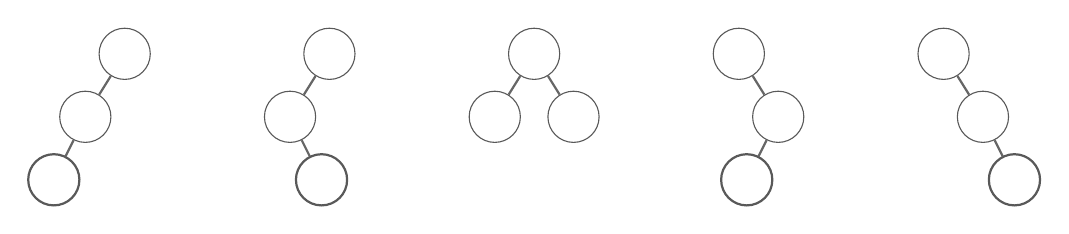
\begin{tikzpicture}[bttree, level distance=8mm, level 1/.style={sibling distance=10mm}, level 2/.style={sibling distance=8mm}]
\node[btn] {} child {node[btn] {} child {node[btn] {}} child[missing]} child[missing];
\begin{scope}[xshift=2.6cm]
\node[btn] {} child {node[btn] {} child[missing] child {node[btn] {}}} child[missing];
\end{scope}
\begin{scope}[xshift=5.2cm]
\node[btn] {} child {node[btn] {}} child {node[btn] {}};
\end{scope}
\begin{scope}[xshift=7.8cm]
\node[btn] {} child[missing] child {node[btn] {} child {node[btn] {}} child[missing]};
\end{scope}
\begin{scope}[xshift=10.4cm]
\node[btn] {} child[missing] child {node[btn] {} child[missing] child {node[btn] {}}};
\end{scope}
\end{tikzpicture}
\diagcaption{$3$ 個節點的二元樹共 $5$ 種形狀。 左邊兩種的左子樹有 $2$ 個節點，中間
那種左右各 $1$ 個，右邊兩種的右子樹有 $2$ 個節點。}
\label{fig:bt-five}
\end{center}

\subsection{遞迴式}

令 $b_n$ 是 $n$ 個節點的二元樹的形狀數。 空樹只有一種，$b_0 = 1$。 $n \ge 1$ 時，
根佔掉一個節點，剩下 $n - 1$ 個分給左右子樹：左子樹 $k$ 個、右子樹 $n - 1 - k$ 個，
$k = 0, 1, \ldots, n - 1$。 左子樹有 $b_k$ 種形狀、右子樹有 $b_{n-1-k}$ 種，任意搭
配，所以
\[
b_n = \sum_{k=0}^{n-1} b_k\, b_{n-1-k}, \qquad b_0 = 1 .
\]
算出來是 $b_1 = 1$、$b_2 = 2$、$b_3 = 2 + 1 + 2 = 5$、$b_4 = 14$、$b_5 = 42$。 這正
是第~6~章出現過的卡特蘭數：

\begin{theorem}
\label{thm:bt-catalan}
$n$ 個節點的二元樹共有 $C_n = \dfrac{1}{n+1}\dbinom{2n}{n}$ 種不同的形狀。
\end{theorem}

\begin{proof}
第~6~章 6.1 節證明了：$1, \ldots, n$ 依序進入堆疊時，做得到的輸出順序有 $C_n$ 種（第~6~
章的定理~6.2），而且這個個數滿足同一個遞迴式 $C_n = \sum_{k=0}^{n-1} C_k\,
C_{n-1-k}$、$C_0 = 1$。 $b_n$ 和 $C_n$ 的起始值和遞迴式都相同，對 $n$ 歸納就得到
$b_n = C_n$。
\end{proof}

第~2~章提過的生成函數也能直接解這個遞迴式：令 $B(x) = \sum_n b_n x^n$，遞迴式等於
$B(x) = 1 + x\,B(x)^2$，解二次方程式再展開，得到同一個公式。 本書不展開這個做法。

\subsection{前序固定時，中序就是堆疊的輸出}

二元樹和堆疊的輸出順序之間，其實有一個直接的對應。 把一棵樹的節點依前序編號
$1, 2, \ldots, n$，再看它的中序。 第~\ref{sec:bt-iter}~節的 \proc{Inorder-Iter} 追
蹤時已經看到：push 的順序是前序，pop（拜訪）的順序是中序。 push 的順序一定是前序，
因為 \proc{Inorder-Iter} 第一次走到一個節點時就 push 它，而它走到節點的順序是根、
整個左子樹、整個右子樹（右子樹要等根 pop 出來才會進去）。 所以\textbf{中序一定是
$1, \ldots, n$ 經過一個堆疊能排出的順序}。 反過來，不同的樹有不同的中序（定
理~\ref{thm:bt-pre-in}），所以「前序是 $1, \ldots, n$ 的樹」對應到的中序兩兩不同，
而這兩邊的個數都是 $C_n$，這個對應是一對一而且映成的。 結論：

\begin{theorem}
\label{thm:bt-pre-stack}
給定前序 $p_1 \cdots p_n$（名稱互不相同），序列 $q_1 \cdots q_n$ 是某一棵前序為
$p_1 \cdots p_n$ 的二元樹的中序，充分必要條件是：$p_1, \ldots, p_n$ 依序 push 進堆
疊、中間隨時可以 pop，pop 出來的順序能夠是 $q_1 \cdots q_n$。 這樣的樹恰好有一棵。
\end{theorem}

這給了一個不用畫樹就能判斷「前序和中序有沒有矛盾」的方法：把前序換成 $1, \ldots,
n$，用第~6~章的定理~6.1 檢查中序裡有沒有「大、小、中」的樣子。 例如前序
$A\,B\,C\,D$、中序 $B\,D\,A\,C$ 換成編號是 $2, 4, 1, 3$，其中 $4, 1, 3$ 是「大、小、
中」，所以沒有這樣的樹，和範例~\ref{ex:bt-rebuild} 的第三組一致。

\subsection{其他用同一個數算的東西}

下面幾種東西的個數也都是卡特蘭數，因為它們都能和二元樹一一對應：

\begin{itemize}
\item \textbf{$n$ 個節點的森林}有 $C_n$ 種：第~\ref{sec:bt-lcrs}~節的轉換是一一對
應。
\item \textbf{$n$ 個節點的有序樹}有 $C_{n-1}$ 種：轉成二元樹後根沒有右孩子，根的
左子樹可以是任何 $n - 1$ 個節點的二元樹。
\item \textbf{有 $n$ 個內部節點的嚴格二元樹}有 $C_n$ 種：把任何一棵 $n$ 個節點的
二元樹的每個 \NIL 都換成一個葉節點（共 $n + 1$ 個），就得到一棵嚴格二元樹，原來的
節點都變成內部節點；反過來把葉節點全部拿掉。 這樣加上葉節點的樹叫\textbf{延伸二元
樹}（extended binary tree），新加的葉節點叫外部節點。
\item \textbf{$n + 1$ 個數連乘、加滿括號}的方法有 $C_n$ 種：每種加法對應一棵有 $n$ 個
運算子（內部節點）、$n + 1$ 個運算元（葉節點）的運算式樹，正是上一項的嚴格二元樹。
\end{itemize}

延伸二元樹的前序，把內部節點寫成 \texttt{1}、外部節點寫成 \texttt{0}，就是範
例~\ref{ex:bt-club} 的延伸前序把字母換成 \texttt{1}、點換成 \texttt{0}。 一串
\texttt{0}、\texttt{1} 是不是某棵樹的延伸前序，可以由左往右數「還要讀幾棵子樹」：一
開始是 $1$；讀到 \texttt{1} 用掉一棵、多出兩棵，淨加一；讀到 \texttt{0} 減一。 合法
的條件是這個數在最後一個字元之前都不是 $0$，最後恰好是 $0$，和第~6~章判斷後序是否合
法的條件是同一類。 用電腦枚舉所有 $n$ 個 \texttt{1}、$n + 1$ 個 \texttt{0} 的字串，數
出合法的個數，就能驗證 $b_n = C_n$。 $C_n$ 成長得很快，大約是
$4^n / (n^{3/2}\sqrt{\pi})$：$C_{10} = 16796$，$C_{20}$ 已經超過六十億。

\section{運算式樹}
\label{sec:bt-expr}

只有二元運算子的運算式可以畫成一棵二元樹：葉節點是運算元，內部節點是運算子，運算
子的左右子樹是它的兩個運算元（各自又是一個運算式）。 這叫\textbf{運算式樹}
（expression tree）。 圖~\ref{fig:bt-expr} 是 $(6 + 2) * 5 - 8 / (3 - 1) \text{\textasciicircum} 2$ 的
運算式樹，\textasciicircum{} 是次方。

\begin{center}
\begin{tikzpicture}[bttree, level 1/.style={sibling distance=40mm}, level 2/.style={sibling distance=20mm}, level 3/.style={sibling distance=12mm}, level 4/.style={sibling distance=9mm}]
\node[btop] {$-$}
    child {node[btop] {$*$}
        child {node[btop] {$+$} child {node[btn] {6}} child {node[btn] {2}}}
        child {node[btn] {5}}}
    child {node[btop] {$/$}
        child {node[btn] {8}}
        child {node[btop] {\textasciicircum}
            child {node[btop] {$-$} child {node[btn] {3}} child {node[btn] {1}}}
            child {node[btn] {2}}}};
\end{tikzpicture}
\diagcaption{$(6 + 2) * 5 - 8 / (3 - 1) \text{\textasciicircum} 2$ 的運算式樹。 橘色是運算子（內部節
點），白色是運算元（葉節點）。 越晚算的運算越靠近根，根是最後算的減法。}
\label{fig:bt-expr}
\end{center}

\subsection{三種走訪就是三種寫法}

第~6~章的前序、中序、後序運算式，就是這棵樹的三種走訪：

\begin{center}
\begin{tabular}{ll}
\toprule
前序走訪（前序式）& $-\;*\;+\;6\;2\;5\;/\;8\;\text{\textasciicircum}\;-\;3\;1\;2$ \\
中序走訪（中序式，要加括號）& $(((6 + 2) * 5) - (8 / ((3 - 1) \text{\textasciicircum} 2)))$ \\
後序走訪（後序式）& $6\;2\;+\;5\;*\;8\;3\;1\;-\;2\;\text{\textasciicircum}\;/\;-$ \\
\bottomrule
\end{tabular}
\end{center}

前序和後序不需要括號：樹的形狀完全由記號的順序決定。 中序就不行了，$6 + 2 * 5$ 可
能是 $(6 + 2) * 5$ 也可能是 $6 + (2 * 5)$，兩棵樹不同，中序走訪卻一樣。 所以從樹印出
中序時要加括號。 最簡單的是每個運算都加（上表那樣），比較好看的做法是只加必要的：
子樹的根是運算子，而且
\begin{itemize}
\item 它的優先順序比父節點低，或
\item 優先順序一樣高，但它在「結合方向的另一邊」：父節點由左往右結合（$+$、$-$、$*$、
$/$）而它是右孩子，或父節點由右往左結合（\textasciicircum）而它是左孩子，
\end{itemize}
就要加括號。 照這個規則，圖~\ref{fig:bt-expr} 印成
$(6 + 2) * 5 - 8 / (3 - 1) \text{\textasciicircum} 2$。 第二條規則對 $+$、$*$ 也加括號，所以
$a + (b + c)$ 會保留括號：數學上它等於 $a + b + c$，但它們是兩棵不同的樹。

注意這裡又看到了定理~\ref{thm:bt-n0n2}：只有二元運算子時，運算式樹是嚴格二元樹，
運算元（葉節點）恰好比運算子多一個。 圖~\ref{fig:bt-expr} 有 $6$ 個運算子、$7$ 個
運算元。

另外，第~\ref{sec:bt-rebuild}~節說前序加後序決定不了一般的二元樹，但一個後序式就能
決定運算式樹，因為看記號就知道每個節點有幾個孩子：運算元是葉節點，二元運算子有兩個
孩子。 這和延伸前序的道理一樣，分支度的資訊已經寫在序列裡了。

\subsection{由後序式建樹與求值}

由左往右讀後序式，堆疊裡放的是「已經建好的子樹」：讀到運算元，建一個葉節點 push；
讀到運算子，pop 出兩棵子樹，\textbf{先 pop 的接在右邊}，接到新的運算子節點下面再
push 回去。 讀完時堆疊裡剩下的唯一一棵就是整棵樹。 這和第~6~章的後序求值是同一個
迴圈，只是堆疊裡放的從「數」換成「樹」。

\begin{pseudo}[label=alg:bt-postfix-tree]{由後序式建運算式樹}
\Function{Postfix-To-Tree}{$T, m$} \Comment{$T[1..m]$ 是記號}
    \State 建立空堆疊 $S$
    \For{$i \gets 1$ \To $m$}
        \State 配置新節點 $x$，$x.\mathit{key} \gets T[i]$
        \If{$T[i]$ 是運算子}
            \State $x.\mathit{right} \gets$ \Call{Pop}{$S$}
            \State $x.\mathit{left} \gets$ \Call{Pop}{$S$}
        \Else
            \State $x.\mathit{left} \gets \NIL$，$x.\mathit{right} \gets \NIL$
        \EndIf
        \State \Call{Push}{$S, x$}
    \EndFor
    \State \Return \Call{Pop}{$S$}
\EndFunction
\end{pseudo}

用 $6\;2\;+\;5\;*\;8\;3\;1\;-\;2\;\text{\textasciicircum}\;/\;-$ 追蹤，堆疊裡的每棵子樹用加滿括號的中
序寫：

\begin{center}
\begin{tabular}{cl}
\toprule
記號 & 之後的堆疊（底 $\to$ 頂，每一項是一棵子樹）\\
\midrule
6, 2 & $6$ \quad $2$ \\
$+$ & $(6 + 2)$ \\
5 & $(6 + 2)$ \quad $5$ \\
$*$ & $((6 + 2) * 5)$ \\
8, 3, 1 & $((6 + 2) * 5)$ \quad $8$ \quad $3$ \quad $1$ \\
$-$ & $((6 + 2) * 5)$ \quad $8$ \quad $(3 - 1)$ \\
2 & $((6 + 2) * 5)$ \quad $8$ \quad $(3 - 1)$ \quad $2$ \\
\textasciicircum & $((6 + 2) * 5)$ \quad $8$ \quad $((3 - 1) \text{\textasciicircum} 2)$ \\
$/$ & $((6 + 2) * 5)$ \quad $(8 / ((3 - 1) \text{\textasciicircum} 2))$ \\
$-$ & $(((6 + 2) * 5) - (8 / ((3 - 1) \text{\textasciicircum} 2)))$ \\
\bottomrule
\end{tabular}
\end{center}

\textbf{求值}就是後序走訪：先算出左右子樹的值，再用根的運算子合起來，葉節點的值是
它自己。 由前序式建樹可以用遞迴（第~6~章 6.3 節前序求值的第二種做法，把「算值」換
成「建節點」）；由中序式建樹，可以先用第~6~章的方法轉成後序，再用上面的迴圈。

\subsection{C 程式}

程式一行讀一個後序式，記號用空白隔開，建好樹之後印出前序式、只加必要括號的中序和值。 不合法的後序式（運算元不夠，或最後剩下不只一棵樹）印出一行訊息。

\begingroup\catcode`\^=12
\begin{example}[label=ex:bt-expr]{c}{(expr\_tree.c) 運算式樹}
#include <stdio.h>
#include <stdlib.h>
#include <string.h>

typedef struct ENode {
    char op;                    // 運算子；運算元時是 0
    long long val;              // 運算元的值
    struct ENode *left, *right;
} ENode;

int prec(char op)
{
    return op == '^' ? 3 : (op == '*' || op == '/') ? 2 : 1;
}

void free_tree(ENode *t)
{
    if (t != NULL) {
        free_tree(t->left);
        free_tree(t->right);
        free(t);
    }
}

// 由後序建樹：運算元 push，運算子 pop 兩棵子樹接起來再 push。
// 不是合法的後序時回傳 NULL。
ENode *build(char *line)
{
    ENode *st[64];
    int top = 0, ok = 1;
    for (char *tok = strtok(line, " \n"); tok != NULL && ok; tok = strtok(NULL, " \n")) {
        ENode *p = malloc(sizeof *p);
        if (p == NULL) {
            exit(1);
        }
        p->left = p->right = NULL;
        if (strchr("+-*/^", tok[0]) != NULL && tok[1] == '\0') {
            p->op = tok[0];
            if (top < 2) {
                ok = 0;             // 運算元不夠
            } else {
                p->right = st[--top];   // 先 pop 出來的是右邊
                p->left = st[--top];
            }
        } else {
            p->op = 0;
            p->val = atoll(tok);
        }
        if (top == 64) {
            ok = 0;
        }
        if (ok) {
            st[top++] = p;
        } else {
            free(p);
        }
    }
    if (ok && top == 1) {
        return st[0];
    }
    while (top > 0) {               // 不合法：把建到一半的子樹都釋放
        free_tree(st[--top]);
    }
    return NULL;
}

void prefix(const ENode *t)
{
    if (t->op) {
        printf(" %c", t->op);
        prefix(t->left);
        prefix(t->right);
    } else {
        printf(" %lld", t->val);
    }
}

// 只加必要的括號：子樹的運算子比較低，或一樣高但結合方向不對
void infix(const ENode *t)
{
    if (!t->op) {
        printf("%lld", t->val);
        return;
    }
    const ENode *l = t->left, *r = t->right;
    int right_assoc = (t->op == '^');
    int pl = l->op && (prec(l->op) < prec(t->op) ||
                       (prec(l->op) == prec(t->op) && right_assoc));
    int pr = r->op && (prec(r->op) < prec(t->op) ||
                       (prec(r->op) == prec(t->op) && !right_assoc));
    if (pl) {
        printf("(");
    }
    infix(l);
    if (pl) {
        printf(")");
    }
    printf(" %c ", t->op);
    if (pr) {
        printf("(");
    }
    infix(r);
    if (pr) {
        printf(")");
    }
}

long long eval(const ENode *t)      // 後序：先算兩邊，再算自己
{
    if (!t->op) {
        return t->val;
    }
    long long a = eval(t->left), b = eval(t->right), r = 1;
    switch (t->op) {
    case '+': return a + b;
    case '-': return a - b;
    case '*': return a * b;
    case '/': return b != 0 ? a / b : 0;    // 範例的資料不會除以 0
    default:
        for (long long i = 0; i < b; i++) {
            r *= a;
        }
        return r;
    }
}

int main(void)
{
    char line[256];
    while (fgets(line, sizeof line, stdin) != NULL) {
        line[strcspn(line, "\n")] = '\0';
        printf("postfix: %s\n", line);
        ENode *root = build(line);
        if (root == NULL) {
            printf("not a valid postfix expression\n");
            continue;
        }
        printf("prefix:");
        prefix(root);
        printf("\ninfix: ");
        infix(root);
        printf("\nvalue: %lld\n", eval(root));
        free_tree(root);
    }
    return 0;
}
\end{example}
\iosample{6 2 + 5 * 8 3 1 - 2 ^ / - \\ 2 3 2 ^ ^ \\ 2 3 ^ 2 ^ \\ 9 4 2 - - \\ 7 + 1}{postfix: 6 2 + 5 * 8 3 1 - 2 ^ / - \\ prefix: - * + 6 2 5 / 8 ^ - 3 1 2 \\ infix: (6 + 2) * 5 - 8 / (3 - 1) ^ 2 \\ value: 38 \\ postfix: 2 3 2 ^ ^ \\ prefix: ^ 2 ^ 3 2 \\ infix: 2 ^ 3 ^ 2 \\ value: 512 \\ postfix: 2 3 ^ 2 ^ \\ prefix: ^ ^ 2 3 2 \\ infix: (2 ^ 3) ^ 2 \\ value: 64 \\ postfix: 9 4 2 - - \\ prefix: - 9 - 4 2 \\ infix: 9 - (4 - 2) \\ value: 7 \\ postfix: 7 + 1 \\ not a valid postfix expression}
\endgroup

第二、三行對照了結合方向：$2 \text{\textasciicircum} 3 \text{\textasciicircum} 2$ 由右往左結合，
樹的右子樹是 $3 \text{\textasciicircum} 2$，印的時候不用括號；左子樹是次方時就要加括號，
值也不同（$512$ 和 $64$）。 第四行的減法由左往右結合，右子樹是減法就要加括號。 最
後一行的 \texttt{7 + 1} 讀到 \texttt{+} 時堆疊裡只有一棵子樹，所以不合法。
\texttt{build} 遇到不合法的輸入時，要把已經建好、還在堆疊裡的子樹都釋放掉，不然
AddressSanitizer 會回報記憶體洩漏。

\section{本章常見錯誤}
\label{sec:bt-pitfalls}

\begin{center}
\begin{tabular}{p{0.22\linewidth}p{0.52\linewidth}p{0.16\linewidth}}
\toprule
錯誤 & 例子 & 見 \\
\midrule
高度差一 & 高度用邊數算，卻套「層數」的公式 $2^h - 1$；空樹和葉節點的高度都寫成 $0$ &
第~\ref{sec:bt-terms}~節 \\
名稱混用 & 把「每個節點 $0$ 或 $2$ 個孩子」當成完整二元樹；沒寫出自己用的定義 &
第~\ref{sec:bt-terms}~節 \\
陣列索引沒換 & C 從 $0$ 開始存，左孩子卻寫 \texttt{2 * i}、父節點寫 \texttt{i / 2} &
第~\ref{sec:bt-array}~節 \\
森林轉換弄反 & 第一個孩子接到右指標、兄弟接到左指標；以為森林的後序對應二元樹的後序 &
第~\ref{sec:bt-lcrs}~節 \\
釋放順序錯 & 先 \texttt{free(t)} 再讀 \texttt{t->left}；只 \texttt{free} 根就以為整棵
樹都釋放了 & 第~\ref{sec:bt-walk}~節 \\
後序迴圈版沒記上一個 & 只看頂端節點有沒有右孩子，右子樹做完回來又走進去一次，變成
無窮迴圈 & 第~\ref{sec:bt-iter}~節 \\
重建時切錯段 & 用中序裡根的位置直接切前序；前序要照左子樹的\textbf{個數}切 &
第~\ref{sec:bt-rebuild}~節 \\
以為前序加後序就夠 & 只有一個孩子的節點，左右看不出來，答案只畫一棵 &
第~\ref{sec:bt-rebuild}~節 \\
引線插入漏一步 & 插在有右子樹的節點下面，沒把後繼的左引線改成指向新節點 &
第~\ref{sec:bt-thread}~節 \\
運算式樹左右顛倒 & 由後序建樹時，先 pop 出來的接在左邊，$8\;3\;-$ 變成 $3 - 8$ &
第~\ref{sec:bt-expr}~節 \\
\bottomrule
\end{tabular}
\end{center}

\section{觀念題}
\label{sec:bt-exercises}

題型和研究所考試、期中期末考的筆試相近，有選擇、計算、追蹤和證明。 解答在本章最後。
題目裡的高度、深度、層數都照第~\ref{sec:bt-terms}~節的定義。

\begin{enumerate}
\item （選擇，可能不只一個答案）下列敘述哪些正確？
\begin{enumerate}
\item 有 $30$ 個葉節點的二元樹，恰好有 $29$ 個分支度為 $2$ 的節點。
\item 有 $100$ 個節點的完整二元樹，高度是 $6$。
\item 高度為 $5$ 的二元樹最多有 $63$ 個節點。
\item 有 $n$ 個節點的二元樹用左右孩子指標存，共有 $n - 1$ 個 \NIL 指標。
\item 節點名稱互不相同時，層序加前序可以唯一決定一棵二元樹。
\end{enumerate}

\item （計算）一棵樹的分支度是 $4$，其中分支度為 $1$、$2$、$3$、$4$ 的節點分別有
$6$、$4$、$3$、$2$ 個。
\begin{enumerate}
\item 這棵樹有幾個葉節點？ 共有幾個節點？
\item 每個節點準備 $4$ 個孩子指標來存，共有幾個空指標？ 改用左孩子右兄弟呢？
\end{enumerate}

\item （計算）一棵 $200$ 個節點的完整二元樹存在 $A[1..200]$。
\begin{enumerate}
\item $A[75]$ 的父節點、左孩子、右孩子在哪一格？ 它的深度是多少？
\item 這棵樹的高度是多少？ 有幾個葉節點？ 有幾個節點恰好只有一個孩子？
\item 改用 C 的 \texttt{a[0..199]} 存，\texttt{a[75]} 的父節點和兩個孩子在哪一格？
\item 一棵完整的三元樹（每個內部節點最多三個孩子，由上到下、由左到右編號）存在
$A[1..n]$。 寫出編號 $i$ 的節點的三個孩子和父節點的編號，並說明理由。
\end{enumerate}

\item \label{q:bt-convert}（追蹤）一棵有序樹寫成 $K(L(P, Q), M, N(R(T), S))$，括號裡是由左到右的
孩子（這一題的括號是一般樹的孩子，不分左右）。
\begin{enumerate}
\item 用左孩子右兄弟轉成二元樹，用本章的 $x(L, R)$ 寫法寫出來。
\item 寫出這棵二元樹的前序和中序，並和原來那棵樹的前序、後序比較。
\end{enumerate}

\item （追蹤）一棵二元樹的前序和中序如下。 畫出這棵樹，寫出它的後序和層序。
\[
\text{前序：}M\,K\,H\,C\,A\,F\,J\,B\,D\,L\,E \qquad
\text{中序：}C\,A\,H\,K\,J\,F\,B\,M\,D\,E\,L
\]

\item （計算）一棵二元樹的前序是 $A\,B\,C\,D\,E$，後序是 $C\,E\,D\,B\,A$。
\begin{enumerate}
\item 符合的二元樹有幾棵？ 全部寫出來。
\item 如果另外知道中序是 $C\,B\,E\,D\,A$，是哪一棵？
\end{enumerate}

\item \label{q:bt-pre-post}（證明）證明定理~\ref{thm:bt-pre-post}：節點名稱互不相同，給
定前序和後序，若至少有一棵二元樹符合，則符合的樹恰好有 $2^m$ 棵，$m$ 是分支度為 $1$
的節點個數。

\item \label{q:bt-level-in}（證明）證明：節點名稱互不相同時，層序和中序可以唯一決定
一棵二元樹。

\item \label{q:bt-stack-height}（證明）證明虛擬碼~\ref{alg:bt-inorder-iter} 執行時，
堆疊裡最多同時有 $h + 1$ 個節點（$h$ 是樹高），並舉一棵會達到 $h + 1$ 的樹。

\item （追蹤）用第~5~題的樹。
\begin{enumerate}
\item 加上中序引線，列出每一條引線（例如「$A$ 的左引線指向 $C$」）。 共有幾條？
\item 用 \proc{In-Succ} 找 $K$、$A$、$B$ 的後繼，用 \proc{In-Pred} 找 $M$ 的前驅。
\item 用 \proc{Insert-Right} 把新節點 $N$ 接成 $H$ 的右孩子，寫出改了哪些指標和旗
標。
\item 接著把新節點 $P$ 接成 $D$ 的右孩子，寫出改了哪些指標和旗標，以及最後的中序。
\end{enumerate}

\item （計算）
\begin{enumerate}
\item $6$ 個節點的二元樹有幾種形狀？
\item 其中根的左子樹恰好有 $2$ 個節點的有幾種？
\item 其中高度是 $5$ 的有幾種？
\item 前序是 $A\,B\,C\,D\,E$ 的二元樹有幾棵？ 其中有沒有中序是 $C\,B\,A\,E\,D$ 的？
有沒有中序是 $C\,A\,B\,E\,D$ 的？ 有的話畫出來。
\end{enumerate}

\item （追蹤）運算式 $(a + b * c) / (d - e) - f * g$。
\begin{enumerate}
\item 畫出運算式樹，寫出前序式和後序式。
\item 用虛擬碼~\ref{alg:bt-postfix-tree} 由後序式建樹，寫出每讀一個記號之後的堆疊
（每棵子樹用加滿括號的中序寫）。
\item $a = 4$、$b = 3$、$c = 2$、$d = 7$、$e = 5$、$f = 1$、$g = 3$ 時，用後序走訪
求值。
\end{enumerate}

\end{enumerate}

\section{實作練習}
\label{sec:bt-practice}

下面是 Aki-Judge 上和本章相關的題目。 很多題只要交一個 \texttt{.c} 檔，實作題目規
定的函式，不寫 \texttt{main}；評測程式會在同一次執行裡呼叫好幾次，所以函式不能依賴
上一次呼叫留下的全域變數，用完的樹也要讓評測程式能逐一 \texttt{free}。

\begin{center}
\begin{tabular}{llc}
\toprule
小節 & 題目 & 難度 \\
\midrule
走訪 & \akiref{build-tree-and-traverse}{建立二元樹並進行各種遍歷} & 基本 \\
 & \akiref{height-and-size}{二元樹的高度與節點數} & 暖身 \\
 & \akiref{level-order-traversal}{二元樹的層序遍歷} & 基本 \\
 & \akiref{inorder-without-recursion}{不用遞迴的中序遍歷} & 基本 \\
 & \akiref{parcel-sorter-gate-tree}{包裹分揀閘門樹} & 基本 \\
 & \akiref{heavier-subtree-first}{重的子樹先走} & 基本 \\
 & \akiref{smallest-overloaded-subtrees}{最小超載子樹} & 進階 \\
 & \akiref{trimmed-copy-symmetric-level-widths}{二元樹的截斷複製、對稱子樹與每層寬度} & 進階 \\
 & \akiref{patch-a-binary-tree}{用修補樹改寫二元樹} & 進階 \\
 & \akiref{lighter-side-first-to-list}{輕的先串：把二元樹改接成雙向串列} & 進階 \\
 & \akiref{deal-deck-into-binary-tree}{輪流發牌建二元樹} & 進階 \\
重建 & \akiref{regrow-tree-from-preorder-record}{照前序紀錄把盆栽種回來} & 基本 \\
 & \akiref{rebuild-from-inorder-depths}{由中序深度還原二元樹} & 進階 \\
一般的樹 & \akiref{folder-tree-paths-sizes-moves}{資料夾樹：路徑、容量與搬移} & 基本 \\
 & \akiref{folder-tree-from-one-line}{一行字串還原資料夾樹} & 進階 \\
 & \akiref{bonsai-pruning-match}{盆栽修剪配對} & 進階 \\
運算式樹 & \akiref{gate-tree-settle-time}{邏輯閘樹的訊號穩定時間} & 進階 \\
\bottomrule
\end{tabular}
\end{center}

幾題的提示：

\begin{itemize}
\item 前四題共用同一個二元樹模組，樹用第~\ref{sec:bt-array}~節的陣列存法給（從 $0$
開始，空格是 $-1$），先轉成指標存法再做。 題目規定空樹的高度是 $0$，和本書的 $-1$
不同。 「不用遞迴的中序遍歷」有一條很長的鏈，要用第~\ref{sec:bt-iter}~節的迴圈版。
\item 「重的子樹先走」「最小超載子樹」先用一次後序算好每棵子樹的總和。 「輕的先串」
是中序的變形，遞迴函式回傳子串列的頭和尾最方便。
\item 「照前序紀錄把盆栽種回來」的紀錄和延伸前序一樣能唯一決定樹，照範
例~\ref{ex:bt-club} 的 \texttt{build} 寫。 「由中序深度還原二元樹」：一段中序裡深度
最小的就是這段的根，照第~\ref{sec:bt-rebuild}~節的方式切開。
\item 「一行字串還原資料夾樹」是左孩子右兄弟；「資料夾樹：路徑、容量與搬移」只給父
節點（第~\ref{sec:bt-lcrs}~節最後）。 「邏輯閘樹的訊號穩定時間」是運算式樹的推廣，
每個閘有很多輸入，求值仍然是後序。
\end{itemize}

\section{讀完你應該會}
\label{sec:bt-checklist}

\begin{itemize}
\item 依指定的定義算出深度、層數、高度，用 $n_0 = n_2 + 1$ 和它對 $k$ 元樹的推廣算
節點數，說出滿、完整、嚴格二元樹的差別。
\item 用陣列存完整二元樹，從 $1$ 或 $0$ 開始都能寫出父節點、孩子的編號；把一般的樹
和森林轉成二元樹，再轉回來。
\item 手寫一棵樹的前序、中序、後序、層序，寫出遞迴版和迴圈版的程式，說出各自用的額
外空間。
\item 由前序（或後序、層序）加中序畫出唯一的樹並寫出每一步；說明前序加後序為什麼不
夠，並算出符合的樹有幾棵。
\item 畫出中序引線，用引線找後繼、前驅，並在引線樹上插入節點。
\item 用卡特蘭數算二元樹、森林、加括號方法的個數；把運算式畫成運算式樹，由後序式建
樹並求值。
\end{itemize}

\textbf{延伸閱讀}（書末會整理完整的參考資料）

\begin{itemize}
\item Thomas H. Cormen 等，\textit{Introduction to Algorithms}，第 4 版，10.3 節（用
指標表示有根樹、左孩子右兄弟）、12.1 節（中序走訪與它的時間）、附錄 B.5 節（樹的名
詞；它的 full、complete 和本書的用詞不同，對照著讀正好練習「先看定義」）。
\item Donald E. Knuth，\textit{The Art of Computer Programming}，Vol.~1，第 3 版，
2.3 節：樹的走訪、引線二元樹、森林和二元樹的對應，本章這幾節的經典出處，寫法嚴謹，
適合想看原始證明的人。
\item Ronald L. Graham、Donald E. Knuth、Oren Patashnik，\textit{Concrete
Mathematics}，第 2 版，7.5 節：用生成函數解出卡特蘭數，就是本章略過的那個做法。
\item Antti Laaksonen，\textit{Competitive Programmer's Handbook}，第 14 章：一般的
樹的走訪、直徑和每個節點的子樹資訊，偏實作。
\item 《C 程式設計基礎》第~19~章 19.14--19.18 節：二元搜尋樹的插入、遍歷、重建與集
合運算，是本書第~9~章的預習。
\end{itemize}

\addcontentsline{toc}{section}{觀念題解答}
\section*{觀念題解答}

\begin{enumerate}
\item (a)、(b)、(c) 正確。 (a)：$n_2 = n_0 - 1 = 29$。 (b)：$\lfloor \lg 100 \rfloor
= 6$（$64 \le 100 < 128$）。 (c)：$2^{5+1} - 1 = 63$。 (d) 錯，是 $n + 1$ 個：$2n$ 個
指標裡只有 $n - 1$ 個指向節點。 (e) 錯：$A(B, -)$ 和 $A(-, B)$ 的層序、前序都是
$A\,B$。

\item
\begin{enumerate}
\item $n_0 = 1 + 1 \cdot n_2 + 2 \cdot n_3 + 3 \cdot n_4 = 1 + 4 + 6 + 6 = 17$。 共
$17 + 6 + 4 + 3 + 2 = 32$ 個節點。 驗算：邊數 $31 = 1 \cdot 6 + 2 \cdot 4 + 3 \cdot 3
+ 4 \cdot 2$。
\item 每個節點 $4$ 個指標：$4 \cdot 32 - 31 = 97$ 個空指標，也就是 $n(k - 1) + 1$。
左孩子右兄弟：$2 \cdot 32 - 31 = 33 = n + 1$ 個。
\end{enumerate}

\item
\begin{enumerate}
\item 父節點 $A[37]$（$\lfloor 75/2 \rfloor$），左孩子 $A[150]$，右孩子 $A[151]$，兩
個都 $\le 200$，存在。 深度 $\lfloor \lg 75 \rfloor = 6$（$64 \le 75 < 128$），在第
$7$ 層。
\item 高度 $\lfloor \lg 200 \rfloor = 7$。 有孩子的節點是 $2i \le 200$ 的那些，即
$i = 1, \ldots, 100$，所以葉節點是 $A[101..200]$，共 $100$ 個。 $A[100]$ 的左孩子是
$A[200]$，右孩子 $A[201]$ 不存在，只有它恰好一個孩子。 驗算：$n_2 = 99$，$n_0 = 100
= n_2 + 1$。
\item 父節點 \texttt{a[37]}（\texttt{(75 - 1) / 2}），孩子 \texttt{a[151]}、
\texttt{a[152]}。 \texttt{a[75]} 是第 $76$ 個節點，和 (a) 不是同一個節點。
\item 依編號順序，每個節點依序「生」三個孩子：節點 $1$ 的孩子是 $2, 3, 4$，節點
$2$ 的是 $5, 6, 7$……。 編號 $1$ 到 $i - 1$ 的節點一共生了 $3(i - 1)$ 個孩子，佔
掉編號 $2$ 到 $3(i - 1) + 1$，所以節點 $i$ 的孩子是 $3i - 1$、$3i$、$3i + 1$。 反過
來，編號 $j \ge 2$ 的父節點是滿足 $3i - 1 \le j \le 3i + 1$ 的 $i$，即
$i = \lfloor (j + 1)/3 \rfloor$。 一般的 $k$ 元樹：孩子是 $k(i - 1) + 2$ 到
$ki + 1$，父節點是 $\lfloor (j - 2)/k \rfloor + 1$。
\end{enumerate}

\item
\begin{enumerate}
\item $K(L(P(-, Q),\, M(-, N(R(T, S), -))),\, -)$。 $L$ 的左孩子 $P$ 是它的第一個孩
子，$P$ 的右孩子 $Q$ 是 $P$ 的弟弟；$L$ 的右邊依序串著 $M$、$N$；$R$ 的左孩子 $T$ 是
$R$ 的孩子，$R$ 的右孩子 $S$ 是 $R$ 的弟弟。
\item 二元樹的前序 $K\,L\,P\,Q\,M\,N\,R\,T\,S$，等於原樹的前序。 二元樹的中序
$P\,Q\,L\,M\,T\,R\,S\,N\,K$，等於原樹的後序（$P, Q$ 做完才輪到 $L$；$T$ 做完輪到
$R$，接著 $S$，再來 $N$，最後是根 $K$）。
\end{enumerate}

\item 根是 $M$，中序切成 $CAHKJFB \,|\, M \,|\, DEL$。 左邊 $7$ 個，前序 $KHCAFJB$：
根 $K$，切成 $CAH \,|\, K \,|\, JFB$；$HCA$ 的根 $H$，左邊 $CA$（根 $C$，$A$ 在右）；
$FJB$ 的根 $F$，左 $J$、右 $B$。 右邊 $DLE$：根 $D$，左邊空，$LE$ 的根 $L$，左孩子
$E$。 樹是
\[
M\bigl(K(H(C(-, A), -), F(J, B)),\; D(-, L(E, -))\bigr).
\]
後序 $A\,C\,H\,J\,B\,F\,K\,E\,L\,D\,M$，層序 $M\,K\,D\,H\,F\,L\,C\,J\,B\,E\,A$。

\item
\begin{enumerate}
\item 根 $A$；前序第二個 $B$ 在後序是第 $4$ 個，所以 $B$ 的子樹有 $4$ 個節點，就是
$A$ 底下全部，$A$ 只有一個孩子。 $B$ 的子樹前序 $BCDE$、後序 $CEDB$：$C$ 在後序是第
$1$ 個，子樹只有 $1$ 個節點，不是全部，所以 $B$ 有兩個孩子，左 $C$、右是前序接著的
$D$。 $D$ 的子樹前序 $DE$、後序 $ED$：只有一個孩子 $E$。 $A$、$D$ 各有左右兩種選
擇，共 $2^2 = 4$ 棵：
$A(B(C, D(E, -)), -)$、$A(B(C, D(-, E)), -)$、$A(-, B(C, D(E, -)))$、
$A(-, B(C, D(-, E)))$。
\item 四棵的中序依序是 $CBEDA$、$CBDEA$、$ACBED$、$ACBDE$，所以是第一棵
$A(B(C, D(E, -)), -)$。
\end{enumerate}

\item 對節點數 $n$ 做強歸納，同時證明「每一棵符合的樹，分支度為 $1$ 的節點都是同一
批」，所以 $m$ 有定義。 設前序 $p_1 \cdots p_n$、後序 $q_1 \cdots q_n$，至少有一棵樹
符合。 $n \le 1$ 時恰好一棵，$m = 0$。

$n \ge 2$：任何符合的樹，根都是 $p_1$，而且根至少有一個孩子。 根的「第一棵子樹」（有
左子樹就是左子樹，否則是右子樹）在前序裡緊接在根後面，所以它的根是 $p_2$；在後序裡
它排在最前面，而且以自己的根結尾，所以若 $p_2 = q_s$，這棵子樹恰好有 $s$ 個節點，前
序是 $p_2 \cdots p_{s+1}$、後序是 $q_1 \cdots q_s$。 $s$ 只由兩個序列決定，和是哪一
棵樹無關。
\begin{itemize}
\item $s = n - 1$：根只有一個孩子，那棵子樹可以接在左邊或右邊。 子問題的符合樹由歸
納假設有 $2^{m'}$ 棵（$m'$ 是子樹裡分支度 $1$ 的節點數，對每棵都一樣），乘上左右兩種
選擇，共 $2^{m'+1}$ 棵，而 $m = m' + 1$（根本身分支度 $1$）。
\item $s < n - 1$：根還有其他子孫，所以有兩個孩子，第一棵子樹必定在左邊。 右子樹的
前序是 $p_{s+2} \cdots p_n$、後序是 $q_{s+1} \cdots q_{n-1}$。 左右兩個子問題各自有
$2^{m_L}$、$2^{m_R}$ 棵，任意搭配，共 $2^{m_L + m_R} = 2^m$ 棵（根的分支度是 $2$，不
算）。
\end{itemize}
兩種情況下，分支度為 $1$ 的節點都由序列決定，歸納完成。 嚴格二元樹 $m = 0$，所以唯
一。

\item 對節點數 $n$ 做強歸納，$n = 0$ 只有空樹。 設層序 $L$、中序 $I$。 根是唯一深度
$0$ 的節點，所以是 $L$ 的第一個 $r$。 名稱互不相同，$r$ 在 $I$ 的位置唯一，左邊的是
左子樹的節點集合 $X$、右邊的是右子樹的 $Y$，左子樹的中序就是 $I$ 裡 $r$ 左邊那一段。
接著說明左子樹的層序就是 $L$ 裡屬於 $X$ 的那些項，順序不變。 層序是先依深度、同一深
度再由左到右排；左子樹裡每個節點的深度都比在整棵樹裡少 $1$，同一深度的節點左右順序
也不變，所以把 $L$ 限制到 $X$ 上，正好是左子樹的層序。 右子樹同理。 兩棵子樹的層序和
中序都由 $L$、$I$ 決定，節點數小於 $n$，由歸納假設唯一，所以整棵樹唯一。

\item 證明下面的不變量：第 4 行每次檢查條件時，堆疊由底到頂 $s_1, \ldots, s_t$ 滿足
每個 $s_{i+1}$ 都在 $s_i$ 的左子樹裡，而且 $x \ne \NIL$、$t \ge 1$ 時，$x$ 在 $s_t$
的左子樹裡。 一開始堆疊是空的，成立。 內層迴圈 push $x$ 之後令
$x \gets x.\mathit{left}$：被 push 的 $x$ 原本就在舊頂端的左子樹裡，新的 $x$ 在它的
左子樹裡，維持住。 第 8--10 行 pop 出 $s_t$、令 $x \gets s_t.\mathit{right}$：新的
$x$ 在 $s_t$ 的子樹裡，而 $s_t$ 在 $s_{t-1}$ 的左子樹裡，所以 $x$ 也在新頂端
$s_{t-1}$ 的左子樹裡，維持住。

由不變量，$s_1, s_2, \ldots, s_t$ 一個是下一個的祖先，全都在從 $s_1$ 往下到 $s_t$ 的
一條路徑上，一條路徑最多 $h + 1$ 個節點，所以 $t \le h + 1$。 只往左長的鏈
（$h + 1$ 個節點）會把整條鏈都 push 進去，達到 $h + 1$。

\item 樹是第~5~題的
\[
M\bigl(K(H(C(-, A), -), F(J, B)),\; D(-, L(E, -))\bigr),
\]
中序 $C\,A\,H\,K\,J\,F\,B\,M\,D\,E\,L$。
\begin{enumerate}
\item 空指標有 $n + 1 = 12$ 個，全都變成引線：$C$ 的左引線（\NIL）；$A$ 左 $\to C$、
右 $\to H$；$H$ 右 $\to K$；$J$ 左 $\to K$、右 $\to F$；$B$ 左 $\to F$、右 $\to M$；
$D$ 左 $\to M$；$E$ 左 $\to D$、右 $\to L$；$L$ 的右引線（\NIL）。 指向節點的有
$10$ 條。
\item $K$ 有右子樹，從 $F$ 往左走到 $J$，$J$ 的左邊是引線，後繼是 $J$。 $A$、$B$ 的
右邊是引線，後繼分別是 $H$、$M$。 $M$ 有左子樹，從 $K$ 往右走：$K \to F \to B$，
$B$ 的右邊是引線，前驅是 $B$。
\item $H$ 的右邊原本是引線（指向 $K$）。 $N.\mathit{right} \gets K$、
$N.\mathit{rthread} \gets \TRUE$；$N.\mathit{left} \gets H$、
$N.\mathit{lthread} \gets \TRUE$；$H.\mathit{right} \gets N$、
$H.\mathit{rthread} \gets \FALSE$。 $N$ 的右邊是引線，不用改別的節點。
\item $D$ 原本有右子樹 $L(E, -)$。 $P.\mathit{right} \gets L$、
$P.\mathit{rthread} \gets \FALSE$；$P.\mathit{left} \gets D$、
$P.\mathit{lthread} \gets \TRUE$；$D.\mathit{right} \gets P$。 $P$ 的後繼是 $L$ 的子
樹最左邊的 $E$，$E$ 的左引線原本指向 $D$，改成指向 $P$。 最後的中序是
$C\,A\,H\,N\,K\,J\,F\,B\,M\,D\,P\,E\,L$。
\end{enumerate}

\item
\begin{enumerate}
\item $C_6 = 132$。
\item 左子樹 $2$ 個、右子樹 $3$ 個：$C_2 \cdot C_3 = 2 \cdot 5 = 10$。
\item 高度 $5$ 表示 $6$ 個節點排成一條路徑，除了根，每個節點是父節點的左孩子或右孩
子，$2^5 = 32$ 種。
\item $C_5 = 42$ 棵。 把 $A, \ldots, E$ 編成 $1, \ldots, 5$：$C\,B\,A\,E\,D$ 是
$3, 2, 1, 5, 4$，沒有「大、小、中」，所以有，而且恰好一棵：根 $A$，左邊 $CB$（$B$
的左孩子 $C$），右邊 $ED$（$D$ 的左孩子 $E$），即 $A(B(C, -), D(E, -))$。
$C\,A\,B\,E\,D$ 是 $3, 1, 2, 5, 4$，含 $3, 1, 2$，所以沒有。
\end{enumerate}

\item
\begin{enumerate}
\item 根是最後算的減法，左子樹是 $(a + b * c) / (d - e)$，右子樹是 $f * g$，寫成
$-\bigl(/(+(a, *(b, c)), -(d, e)),\; *(f, g)\bigr)$。 前序式
$-\;/\;+\;a\;*\;b\;c\;-\;d\;e\;*\;f\;g$，後序式
$a\;b\;c\;*\;+\;d\;e\;-\;/\;f\;g\;*\;-$。
\item 依序：$a$；$a$ $b$；$a$ $b$ $c$；$*$ 之後 $a$ $(b * c)$；$+$ 之後
$(a + (b * c))$；$d$、$e$ 之後 $(a + (b * c))$ $d$ $e$；$-$ 之後 $(a + (b * c))$
$(d - e)$；$/$ 之後 $((a + (b * c)) / (d - e))$；$f$、$g$ 之後再多兩項 $f$ $g$；$*$
之後 $((a + (b * c)) / (d - e))$ $(f * g)$；$-$ 之後剩下一棵
$(((a + (b * c)) / (d - e)) - (f * g))$。
\item $b * c = 6$，$a + 6 = 10$，$d - e = 2$，$10 / 2 = 5$，$f * g = 3$，$5 - 3 = 2$。
\end{enumerate}

\end{enumerate}
